
% Default to the notebook output style

    


% Inherit from the specified cell style.




    
\documentclass{article}

    
    
    \usepackage{graphicx} % Used to insert images
    \usepackage{adjustbox} % Used to constrain images to a maximum size 
    \usepackage{color} % Allow colors to be defined
    \usepackage{enumerate} % Needed for markdown enumerations to work
    \usepackage{geometry} % Used to adjust the document margins
    \usepackage{amsmath} % Equations
    \usepackage{amssymb} % Equations
    \usepackage[mathletters]{ucs} % Extended unicode (utf-8) support
    \usepackage[utf8x]{inputenc} % Allow utf-8 characters in the tex document
    \usepackage{fancyvrb} % verbatim replacement that allows latex
    \usepackage{grffile} % extends the file name processing of package graphics 
                         % to support a larger range 
    % The hyperref package gives us a pdf with properly built
    % internal navigation ('pdf bookmarks' for the table of contents,
    % internal cross-reference links, web links for URLs, etc.)
    \usepackage{hyperref}
    \usepackage{longtable} % longtable support required by pandoc >1.10
    \usepackage{booktabs}  % table support for pandoc > 1.12.2
		%\usepackage[bitstream-charter]{mathdesign}
		%\usepackage[urw-garamond]{mathdesign}
    \usepackage{tgpagella}
		\usepackage{eulervm}
    

	
    \definecolor{orange}{cmyk}{0,0.4,0.8,0.2}
    \definecolor{darkorange}{rgb}{.71,0.21,0.01}
    \definecolor{darkgreen}{rgb}{.12,.54,.11}
    \definecolor{myteal}{rgb}{.26, .44, .56}
    \definecolor{gray}{gray}{0.45}
    \definecolor{lightgray}{gray}{.95}
    \definecolor{mediumgray}{gray}{.8}
    \definecolor{inputbackground}{rgb}{.95, .95, .85}
    \definecolor{outputbackground}{rgb}{.95, .95, .95}
    \definecolor{traceback}{rgb}{1, .95, .95}
    % ansi colors
    \definecolor{red}{rgb}{.6,0,0}
    \definecolor{green}{rgb}{0,.65,0}
    \definecolor{brown}{rgb}{0.6,0.6,0}
    \definecolor{blue}{rgb}{0,.145,.698}
    \definecolor{purple}{rgb}{.698,.145,.698}
    \definecolor{cyan}{rgb}{0,.698,.698}
    \definecolor{lightgray}{gray}{0.5}
    
    % bright ansi colors
    \definecolor{darkgray}{gray}{0.25}
    \definecolor{lightred}{rgb}{1.0,0.39,0.28}
    \definecolor{lightgreen}{rgb}{0.48,0.99,0.0}
    \definecolor{lightblue}{rgb}{0.53,0.81,0.92}
    \definecolor{lightpurple}{rgb}{0.87,0.63,0.87}
    \definecolor{lightcyan}{rgb}{0.5,1.0,0.83}
    


    % commands and environments needed by pandoc snippets
    % extracted from the output of `pandoc -s`
    \DefineVerbatimEnvironment{Highlighting}{Verbatim}{commandchars=\\\{\},fontsize=\small}
    % Add ',fontsize=\small' for more characters per line
    \newenvironment{Shaded}{}{}
    \newcommand{\KeywordTok}[1]{\textcolor[rgb]{0.00,0.44,0.13}{\textbf{{#1}}}}
    \newcommand{\DataTypeTok}[1]{\textcolor[rgb]{0.56,0.13,0.00}{{#1}}}
    \newcommand{\DecValTok}[1]{\textcolor[rgb]{0.25,0.63,0.44}{{#1}}}
    \newcommand{\BaseNTok}[1]{\textcolor[rgb]{0.25,0.63,0.44}{{#1}}}
    \newcommand{\FloatTok}[1]{\textcolor[rgb]{0.25,0.63,0.44}{{#1}}}
    \newcommand{\CharTok}[1]{\textcolor[rgb]{0.25,0.44,0.63}{{#1}}}
    \newcommand{\StringTok}[1]{\textcolor[rgb]{0.25,0.44,0.63}{{#1}}}
    \newcommand{\CommentTok}[1]{\textcolor[rgb]{0.38,0.63,0.69}{\textit{{#1}}}}
    \newcommand{\OtherTok}[1]{\textcolor[rgb]{0.00,0.44,0.13}{{#1}}}
    \newcommand{\AlertTok}[1]{\textcolor[rgb]{1.00,0.00,0.00}{\textbf{{#1}}}}
    \newcommand{\FunctionTok}[1]{\textcolor[rgb]{0.02,0.16,0.49}{{#1}}}
    \newcommand{\RegionMarkerTok}[1]{{#1}}
    \newcommand{\ErrorTok}[1]{\textcolor[rgb]{1.00,0.00,0.00}{\textbf{{#1}}}}
    \newcommand{\NormalTok}[1]{{#1}}
    
    % Define a nice break command that doesn't care if a line doesn't already
    % exist.
    \def\br{\hspace*{\fill} \\* }
    % Math Jax compatability definitions
    \def\gt{>}
    \def\lt{<}
    % Document parameters
    \title{Introduction to The Finite Element Method using Python}
    \author{Arthur B. Soprano}
    
    

    % Pygments definitions
    
\makeatletter
\def\PY@reset{\let\PY@it=\relax \let\PY@bf=\relax%
    \let\PY@ul=\relax \let\PY@tc=\relax%
    \let\PY@bc=\relax \let\PY@ff=\relax}
\def\PY@tok#1{\csname PY@tok@#1\endcsname}
\def\PY@toks#1+{\ifx\relax#1\empty\else%
    \PY@tok{#1}\expandafter\PY@toks\fi}
\def\PY@do#1{\PY@bc{\PY@tc{\PY@ul{%
    \PY@it{\PY@bf{\PY@ff{#1}}}}}}}
\def\PY#1#2{\PY@reset\PY@toks#1+\relax+\PY@do{#2}}

\expandafter\def\csname PY@tok@gd\endcsname{\def\PY@tc##1{\textcolor[rgb]{0.63,0.00,0.00}{##1}}}
\expandafter\def\csname PY@tok@gu\endcsname{\let\PY@bf=\textbf\def\PY@tc##1{\textcolor[rgb]{0.50,0.00,0.50}{##1}}}
\expandafter\def\csname PY@tok@gt\endcsname{\def\PY@tc##1{\textcolor[rgb]{0.00,0.27,0.87}{##1}}}
\expandafter\def\csname PY@tok@gs\endcsname{\let\PY@bf=\textbf}
\expandafter\def\csname PY@tok@gr\endcsname{\def\PY@tc##1{\textcolor[rgb]{1.00,0.00,0.00}{##1}}}
\expandafter\def\csname PY@tok@cm\endcsname{\let\PY@it=\textit\def\PY@tc##1{\textcolor[rgb]{0.25,0.50,0.50}{##1}}}
\expandafter\def\csname PY@tok@vg\endcsname{\def\PY@tc##1{\textcolor[rgb]{0.10,0.09,0.49}{##1}}}
\expandafter\def\csname PY@tok@m\endcsname{\def\PY@tc##1{\textcolor[rgb]{0.40,0.40,0.40}{##1}}}
\expandafter\def\csname PY@tok@mh\endcsname{\def\PY@tc##1{\textcolor[rgb]{0.40,0.40,0.40}{##1}}}
\expandafter\def\csname PY@tok@go\endcsname{\def\PY@tc##1{\textcolor[rgb]{0.53,0.53,0.53}{##1}}}
\expandafter\def\csname PY@tok@ge\endcsname{\let\PY@it=\textit}
\expandafter\def\csname PY@tok@vc\endcsname{\def\PY@tc##1{\textcolor[rgb]{0.10,0.09,0.49}{##1}}}
\expandafter\def\csname PY@tok@il\endcsname{\def\PY@tc##1{\textcolor[rgb]{0.40,0.40,0.40}{##1}}}
\expandafter\def\csname PY@tok@cs\endcsname{\let\PY@it=\textit\def\PY@tc##1{\textcolor[rgb]{0.25,0.50,0.50}{##1}}}
\expandafter\def\csname PY@tok@cp\endcsname{\def\PY@tc##1{\textcolor[rgb]{0.74,0.48,0.00}{##1}}}
\expandafter\def\csname PY@tok@gi\endcsname{\def\PY@tc##1{\textcolor[rgb]{0.00,0.63,0.00}{##1}}}
\expandafter\def\csname PY@tok@gh\endcsname{\let\PY@bf=\textbf\def\PY@tc##1{\textcolor[rgb]{0.00,0.00,0.50}{##1}}}
\expandafter\def\csname PY@tok@ni\endcsname{\let\PY@bf=\textbf\def\PY@tc##1{\textcolor[rgb]{0.60,0.60,0.60}{##1}}}
\expandafter\def\csname PY@tok@nl\endcsname{\def\PY@tc##1{\textcolor[rgb]{0.63,0.63,0.00}{##1}}}
\expandafter\def\csname PY@tok@nn\endcsname{\let\PY@bf=\textbf\def\PY@tc##1{\textcolor[rgb]{0.00,0.00,1.00}{##1}}}
\expandafter\def\csname PY@tok@no\endcsname{\def\PY@tc##1{\textcolor[rgb]{0.53,0.00,0.00}{##1}}}
\expandafter\def\csname PY@tok@na\endcsname{\def\PY@tc##1{\textcolor[rgb]{0.49,0.56,0.16}{##1}}}
\expandafter\def\csname PY@tok@nb\endcsname{\def\PY@tc##1{\textcolor[rgb]{0.00,0.50,0.00}{##1}}}
\expandafter\def\csname PY@tok@nc\endcsname{\let\PY@bf=\textbf\def\PY@tc##1{\textcolor[rgb]{0.00,0.00,1.00}{##1}}}
\expandafter\def\csname PY@tok@nd\endcsname{\def\PY@tc##1{\textcolor[rgb]{0.67,0.13,1.00}{##1}}}
\expandafter\def\csname PY@tok@ne\endcsname{\let\PY@bf=\textbf\def\PY@tc##1{\textcolor[rgb]{0.82,0.25,0.23}{##1}}}
\expandafter\def\csname PY@tok@nf\endcsname{\def\PY@tc##1{\textcolor[rgb]{0.00,0.00,1.00}{##1}}}
\expandafter\def\csname PY@tok@si\endcsname{\let\PY@bf=\textbf\def\PY@tc##1{\textcolor[rgb]{0.73,0.40,0.53}{##1}}}
\expandafter\def\csname PY@tok@s2\endcsname{\def\PY@tc##1{\textcolor[rgb]{0.73,0.13,0.13}{##1}}}
\expandafter\def\csname PY@tok@vi\endcsname{\def\PY@tc##1{\textcolor[rgb]{0.10,0.09,0.49}{##1}}}
\expandafter\def\csname PY@tok@nt\endcsname{\let\PY@bf=\textbf\def\PY@tc##1{\textcolor[rgb]{0.00,0.50,0.00}{##1}}}
\expandafter\def\csname PY@tok@nv\endcsname{\def\PY@tc##1{\textcolor[rgb]{0.10,0.09,0.49}{##1}}}
\expandafter\def\csname PY@tok@s1\endcsname{\def\PY@tc##1{\textcolor[rgb]{0.73,0.13,0.13}{##1}}}
\expandafter\def\csname PY@tok@sh\endcsname{\def\PY@tc##1{\textcolor[rgb]{0.73,0.13,0.13}{##1}}}
\expandafter\def\csname PY@tok@sc\endcsname{\def\PY@tc##1{\textcolor[rgb]{0.73,0.13,0.13}{##1}}}
\expandafter\def\csname PY@tok@sx\endcsname{\def\PY@tc##1{\textcolor[rgb]{0.00,0.50,0.00}{##1}}}
\expandafter\def\csname PY@tok@bp\endcsname{\def\PY@tc##1{\textcolor[rgb]{0.00,0.50,0.00}{##1}}}
\expandafter\def\csname PY@tok@c1\endcsname{\let\PY@it=\textit\def\PY@tc##1{\textcolor[rgb]{0.25,0.50,0.50}{##1}}}
\expandafter\def\csname PY@tok@kc\endcsname{\let\PY@bf=\textbf\def\PY@tc##1{\textcolor[rgb]{0.00,0.50,0.00}{##1}}}
\expandafter\def\csname PY@tok@c\endcsname{\let\PY@it=\textit\def\PY@tc##1{\textcolor[rgb]{0.25,0.50,0.50}{##1}}}
\expandafter\def\csname PY@tok@mf\endcsname{\def\PY@tc##1{\textcolor[rgb]{0.40,0.40,0.40}{##1}}}
\expandafter\def\csname PY@tok@err\endcsname{\def\PY@bc##1{\setlength{\fboxsep}{0pt}\fcolorbox[rgb]{1.00,0.00,0.00}{1,1,1}{\strut ##1}}}
\expandafter\def\csname PY@tok@kd\endcsname{\let\PY@bf=\textbf\def\PY@tc##1{\textcolor[rgb]{0.00,0.50,0.00}{##1}}}
\expandafter\def\csname PY@tok@ss\endcsname{\def\PY@tc##1{\textcolor[rgb]{0.10,0.09,0.49}{##1}}}
\expandafter\def\csname PY@tok@sr\endcsname{\def\PY@tc##1{\textcolor[rgb]{0.73,0.40,0.53}{##1}}}
\expandafter\def\csname PY@tok@mo\endcsname{\def\PY@tc##1{\textcolor[rgb]{0.40,0.40,0.40}{##1}}}
\expandafter\def\csname PY@tok@kn\endcsname{\let\PY@bf=\textbf\def\PY@tc##1{\textcolor[rgb]{0.00,0.50,0.00}{##1}}}
\expandafter\def\csname PY@tok@mi\endcsname{\def\PY@tc##1{\textcolor[rgb]{0.40,0.40,0.40}{##1}}}
\expandafter\def\csname PY@tok@gp\endcsname{\let\PY@bf=\textbf\def\PY@tc##1{\textcolor[rgb]{0.00,0.00,0.50}{##1}}}
\expandafter\def\csname PY@tok@o\endcsname{\def\PY@tc##1{\textcolor[rgb]{0.40,0.40,0.40}{##1}}}
\expandafter\def\csname PY@tok@kr\endcsname{\let\PY@bf=\textbf\def\PY@tc##1{\textcolor[rgb]{0.00,0.50,0.00}{##1}}}
\expandafter\def\csname PY@tok@s\endcsname{\def\PY@tc##1{\textcolor[rgb]{0.73,0.13,0.13}{##1}}}
\expandafter\def\csname PY@tok@kp\endcsname{\def\PY@tc##1{\textcolor[rgb]{0.00,0.50,0.00}{##1}}}
\expandafter\def\csname PY@tok@w\endcsname{\def\PY@tc##1{\textcolor[rgb]{0.73,0.73,0.73}{##1}}}
\expandafter\def\csname PY@tok@kt\endcsname{\def\PY@tc##1{\textcolor[rgb]{0.69,0.00,0.25}{##1}}}
\expandafter\def\csname PY@tok@ow\endcsname{\let\PY@bf=\textbf\def\PY@tc##1{\textcolor[rgb]{0.67,0.13,1.00}{##1}}}
\expandafter\def\csname PY@tok@sb\endcsname{\def\PY@tc##1{\textcolor[rgb]{0.73,0.13,0.13}{##1}}}
\expandafter\def\csname PY@tok@k\endcsname{\let\PY@bf=\textbf\def\PY@tc##1{\textcolor[rgb]{0.00,0.50,0.00}{##1}}}
\expandafter\def\csname PY@tok@se\endcsname{\let\PY@bf=\textbf\def\PY@tc##1{\textcolor[rgb]{0.73,0.40,0.13}{##1}}}
\expandafter\def\csname PY@tok@sd\endcsname{\let\PY@it=\textit\def\PY@tc##1{\textcolor[rgb]{0.73,0.13,0.13}{##1}}}

\def\PYZbs{\char`\\}
\def\PYZus{\char`\_}
\def\PYZob{\char`\{}
\def\PYZcb{\char`\}}
\def\PYZca{\char`\^}
\def\PYZam{\char`\&}
\def\PYZlt{\char`\<}
\def\PYZgt{\char`\>}
\def\PYZsh{\char`\#}
\def\PYZpc{\char`\%}
\def\PYZdl{\char`\$}
\def\PYZhy{\char`\-}
\def\PYZsq{\char`\'}
\def\PYZdq{\char`\"}
\def\PYZti{\char`\~}
% for compatibility with earlier versions
\def\PYZat{@}
\def\PYZlb{[}
\def\PYZrb{]}
\makeatother


    % Exact colors from NB
    \definecolor{incolor}{rgb}{0.0, 0.0, 0.5}
    \definecolor{outcolor}{rgb}{0.545, 0.0, 0.0}



    
    % Prevent overflowing lines due to hard-to-break entities
    \sloppy 
    % Setup hyperref package
    \hypersetup{
      breaklinks=true,  % so long urls are correctly broken across lines
      colorlinks=true,
      urlcolor=blue,
      linkcolor=darkorange,
      citecolor=darkgreen,
      }
    % Slightly bigger margins than the latex defaults
    
    \geometry{verbose,tmargin=1in,bmargin=1in,lmargin=1in,rmargin=1in}
    
    

    \begin{document}
    
    
    \maketitle
    
    

    
    \section{Finite Elements Notebook}\label{finite-elements-notebook}

\emph{by Arthur B. Soprano - arthursoprano@gmail.com}

\emph{Class notes from Professor Giuseppe Gambolati and Professor Carlo
Janna: \textbf{Solving Geomechanical Problems with the Finite Element
Method}. Special thanks to Jaime Ambrus and Edson Tadeu Manoel for
helping with the class notes.}

    This notebook intends to give a brief review and a short example of the
\textbf{Finite Element Method - FEM} using Python programming language.
First, let's import the necessary packages. For our analysis, we'll need
\href{http://www.numpy.org/}{numpy} and
\href{http://matplotlib.org/}{matplotlib}. Also, we'll define the images
to be showed in this notebook.


    \begin{Verbatim}[commandchars=\\\{\}]
{\color{incolor}In [{\color{incolor}1}]:} \PY{k+kn}{import} \PY{n+nn}{numpy} \PY{k+kn}{as} \PY{n+nn}{np}
        \PY{k+kn}{import} \PY{n+nn}{matplotlib.pyplot} \PY{k+kn}{as} \PY{n+nn}{plt}
        
        \PY{k+kn}{from} \PY{n+nn}{IPython.display} \PY{k+kn}{import} \PY{n}{Image}
        \PY{n}{image1} \PY{o}{=} \PY{n}{Image}\PY{p}{(}\PY{n}{filename}\PY{o}{=}\PY{l+s}{\PYZsq{}}\PY{l+s}{images/square\PYZus{}summable.jpg}\PY{l+s}{\PYZsq{}}\PY{p}{)}
        \PY{n}{image2} \PY{o}{=} \PY{n}{Image}\PY{p}{(}\PY{n}{filename}\PY{o}{=}\PY{l+s}{\PYZsq{}}\PY{l+s}{images/triangle\PYZus{}fe.jpg}\PY{l+s}{\PYZsq{}}\PY{p}{)}
        
        \PY{c}{\PYZsh{} Remove this line for a pop\PYZhy{}up (qt) plot}
        \PY{o}{\PYZpc{}}\PY{k}{matplotlib} \PY{n}{inline} 
\end{Verbatim}

    \section{Indroduction}\label{indroduction}

\subsection{Variational Principles}\label{variational-principles}

We say that a variational principle exists if the solution to a
(generally well behaved) problem is obtained through the
\textbf{minimization} of \textgreater{} an integral expression =
functional = variational principle

Tipically the wanted solution is subject to boundary conditions, so we
are in fact looking for a \textbf{constrained minimum}.

\subsection{Functional Minimization
Methods}\label{functional-minimization-methods}

Minimization of the variational principle \(\Omega\) is performed with
the aid of a functional linear space. The items of a linear space are
\textbf{functions}. The \textbf{norm} of a function \(f\) is defined as
(in a one-dimensional space):

\[
    \left\lVert f \right\rVert = \sqrt{\int^{b}_{a}{f^{2}(x)}\, \mathrm{d}x} = \text{Euclidean "norm"}
\]

If the above norm exists for any space fucntion the space is said to be
\textbf{measurable} and the norm of \(f\) is assumed to be the
\textbf{measure} of \(f\). The scalar product between \(f_1\) and
\(f_2\) is defined as:

\[
    \int^{b}_{a}{f_1(x)f_2(x)}\, \mathrm{d}x \neq \infty
\]

if the space is \textbf{measurable} and if

\[
    \int^{b}_{a}{f_1(x)f_2(x)}\, \mathrm{d}x = 0
\]

the functions \(f_1\) and \(f_2\) are said to be \textbf{orthogonal}.

The functional space made of all functions which have finite Euclidean
norm is denoted by \(L_2\). The functional space \(L_2\) is made of all
the functions which are \textbf{square summable}.

\begin{figure}[h!]
	\centering
		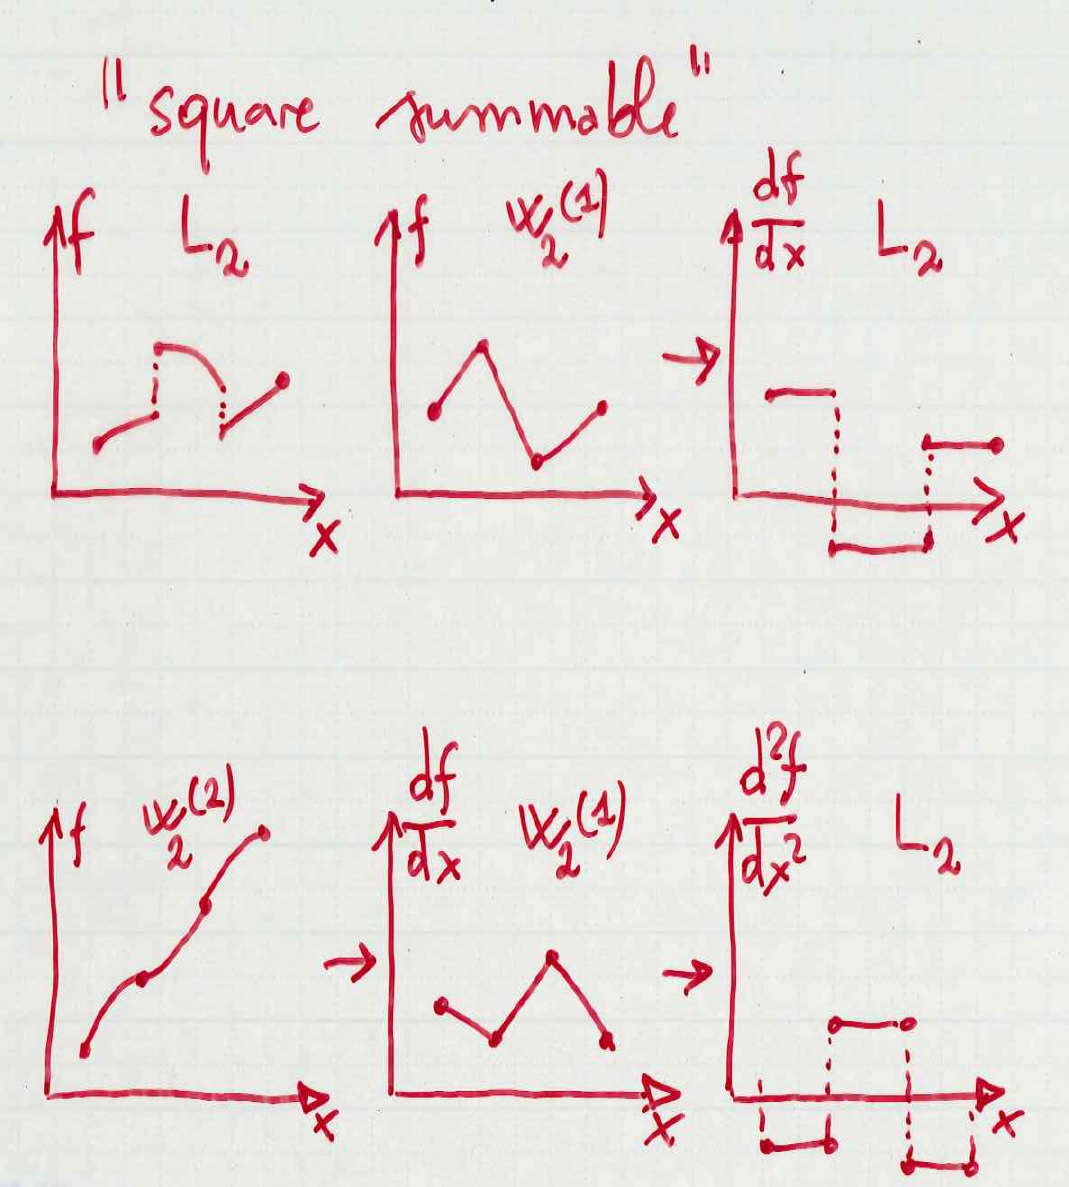
\includegraphics[width=0.7\textwidth]{./images/square_summable.jpg}
	\caption{Examples of square summable fucntions.}
	\label{fig:square_summable}
\end{figure}
    

    If we prescribe restrictions on the continuity of the derivatives of the
space we get \textbf{higher order spaces} called \textbf{Sobolev
spaces}. The Sobolev spaces are subspaces of \(L_2\). For example,
\(W^{(1)}_2\) is the space made by all the functions whose first
derivatives are also square summable

\[
\sqrt{\int^{b}_{a}{f^{2} + \left(\frac{\partial f}{\partial x}\right)^2}\, \mathrm{d}x} \neq \infty
\]

Similarly, \(W^{(2)}_2\) is the space made by all the functions whose
first and second order derivatives are square summable

\[
\sqrt{\int^{b}_{a}{f^{2} + \left(\frac{\partial f}{\partial x}\right)^2 + \left(\frac{\partial^2 f}{\partial x^2}\right)^2}\, \mathrm{d}x} \neq \infty
\]

Higher order spaces are subsets of lower order spaces, i.e., they are
\textbf{subspaces} of lower spaces. The lowest possible space is
\(L_2\), which contains all the Sobolev spaces
\(W^{(1)}_2,W^{(2)}_2,\ldots,W^{(k)}_2\).

\subsection{\texorpdfstring{Approximation of a Function in
\(L_2\)}{Approximation of a Function in L\_2}}\label{approximation-of-a-function-in-lux5f2}

We first identify a (generally) infinite set of functions
\(\xi_1, \xi_2, \ldots, \xi_n\) belonging to \(L_2\) that defines a
\textbf{basis}. For \(\xi_1, \xi_2, \ldots, \xi_n\) to represent a
basis, it is mandatory that for any given function \(f\) of \(L_2\) and
any given (small) number \(\epsilon\) the exists an \(n\) (depending on
\(\epsilon\)) and a set of coefficient \(a_1, a_2, \ldots, a_n\) such
that the linear combination \(f_n\) given by

\[
f_n = a_1 \xi_1 + a_2 \xi_2 + \ldots + a_n \xi_n
\]

differs from \(f\) less than \(\epsilon\), namely

\[
\left\lVert f - f_n \right\rVert < \epsilon
\]

Notice that the set \(\xi_1, \xi_2, \ldots, \xi_n\) defines a subspace
\(S_n\) of the full space \(L_2\). It is intuitive that as \(n\)
increases \(S_n\) approximates \(L_2\) better and better with
\(S_n \rightarrow L_2\) as \(n \rightarrow \infty\).

\section{Ritz FEM Method}\label{ritz-fem-method}

The \textbf{Ritz FEM} method looks for an approximation \(\bar{u}_n\) to
the solution of the variational problem (i.e., the minimizing function
\(\bar{u}\)) with the aid of an \(L_2\) basis:

\[
\bar{u}_n = a_1 \xi_1 + a_2 \xi_2 + \ldots + a_n \xi_n
\]

where \(\xi_1, \xi_2, \ldots, \xi_n\) are the \textbf{basis functions}.
We consider the functional \(\Omega(\bar{u}_n)\) in the space \(S_n\)
and minimize it in \(S_n\):

\[
\frac{\partial \Omega}{\partial a_i}(\bar{u}_n) = 0
\]

for \(i=1,2,\ldots,n\), giving rise to \(n\) algebraic equations that
are linear if \(\Omega\) is a quadratic functional.

\subsection{Example of FEM}\label{example-of-fem}

In order to understand the Ritz FEM method, let's consider the following
example

\[
\Omega(\bar{u}_n) = \int^{1}_{0}\left[\frac{1}{2}(u')^2 + \alpha u\right]\, \mathrm{d}x 
\]

subject to \(u(0)=u(1)=0\) boundary conditions. Select a polinomial
basis:

\[
1, x, x^2, x^3, \ldots
\]

Now let's look for the approximate solution

\[
\bar{u}_n = x(1-x) \sum^{n}_{i=1}a_i x^{i-1}
\]

which satisfies \emph{a priori} the boundary conditions. The lowest
order approximation (\(n = 1\)) is

\[
u_1 = a_1 x (1-x)
\]

Replace \(u_1\) in \(\Omega(\bar{u}_n)\) and differentiate with respect
to \(a_1\):

\[
\frac{\partial \Omega}{\partial a_i} = \frac{\partial}{\partial a_i} \int^1_0\left[\frac{1}{2} a^{2}_{1} (1-2x)^2 + \alpha a_1 x (1-x) \right] \, \mathrm{d}x = 0 
\] \[
\int^1_0\left[a_1 (1-2x)^2 + \alpha x (1-x) \right] \, \mathrm{d}x = 0
\] \[
a_1 = -\frac{\alpha}{2}
\] \[
u_1 = -\frac{\alpha}{2}x(1-x)
\]

Is is easily shown that with \(n>1\) we would get
\(a_2=a_3=\ldots=a_n=0\), i.e.,

\[
u_1 = -\frac{\alpha}{2}x(1-x)=\text{analytical solution}
\]

Select this other basis:

\[
a_n = \sum^n_{i=1} a_i sin(i \pi x)
\]

satisfying the boundary conditions. Let's choose
\(u_1 = a_1 sin(\pi x)\) and minimize \(\Omega(a_1)\):

\[
\frac{\partial \Omega}{\partial a_i} = \frac{\partial}{\partial a_i} \int^1_0\left[\frac{1}{2} a^{2}_{1} \pi^2 cos^2(\pi x) + \alpha a_1 sin(\pi x) \right] \, \mathrm{d}x = 0 
\] \[
\int^1_0\left[a_{1} \pi^2 cos^2(\pi x) + \alpha sin(\pi x) \right] \, \mathrm{d}x = 0 
\] \[
a_1 = -\frac{4 \alpha}{\pi^3}
\] \[
u_1 = -\frac{4 \alpha}{\pi^3}sin(\pi x)
\]

We can compare the two approximations and check that they have similar
values:

    \begin{Verbatim}[commandchars=\\\{\}]
{\color{incolor}In [{\color{incolor}3}]:} \PY{c}{\PYZsh{} Numerical example}
        \PY{n}{x} \PY{o}{=} \PY{n}{np}\PY{o}{.}\PY{n}{array}\PY{p}{(}\PY{p}{[}\PY{l+m+mf}{0.0}\PY{p}{,} \PY{l+m+mf}{0.25}\PY{p}{,} \PY{l+m+mf}{0.5}\PY{p}{,} \PY{l+m+mf}{1.0}\PY{p}{]}\PY{p}{)}
        \PY{n}{alpha} \PY{o}{=} \PY{l+m+mf}{1.0}
        \PY{n}{u1} \PY{o}{=} \PY{o}{\PYZhy{}}\PY{l+m+mf}{0.5} \PY{o}{*} \PY{n}{alpha} \PY{o}{*} \PY{n}{x} \PY{o}{*} \PY{p}{(}\PY{l+m+mi}{1} \PY{o}{\PYZhy{}} \PY{n}{x}\PY{p}{)}
        \PY{n}{u2} \PY{o}{=} \PY{o}{\PYZhy{}}\PY{p}{(}\PY{l+m+mf}{4.0} \PY{o}{*} \PY{n}{alpha} \PY{o}{/} \PY{p}{(}\PY{n}{np}\PY{o}{.}\PY{n}{pi} \PY{o}{*}\PY{o}{*} \PY{l+m+mi}{3}\PY{p}{)}\PY{p}{)} \PY{o}{*} \PY{n}{np}\PY{o}{.}\PY{n}{sin}\PY{p}{(}\PY{n}{np}\PY{o}{.}\PY{n}{pi}\PY{o}{*}\PY{n}{x}\PY{p}{)}
        \PY{k}{print} \PY{l+s}{\PYZdq{}}\PY{l+s}{  x  |   u1   |   u1 (sin())}\PY{l+s}{\PYZdq{}}
        \PY{k}{for} \PY{n}{c1}\PY{p}{,} \PY{n}{c2}\PY{p}{,} \PY{n}{c3} \PY{o+ow}{in} \PY{n+nb}{zip}\PY{p}{(}\PY{n}{x}\PY{p}{,} \PY{n}{u1}\PY{p}{,} \PY{n}{u2}\PY{p}{)}\PY{p}{:}  
            \PY{k}{print} \PY{l+s}{\PYZdq{}}\PY{l+s+si}{\PYZpc{}.2f}\PY{l+s}{ | }\PY{l+s+si}{\PYZpc{}.3f}\PY{l+s}{ | }\PY{l+s+si}{\PYZpc{}.3f}\PY{l+s}{\PYZdq{}} \PY{o}{\PYZpc{}} \PY{p}{(}\PY{n}{c1}\PY{p}{,} \PY{n}{c2}\PY{p}{,} \PY{n}{c3}\PY{p}{)}
\end{Verbatim}

    \begin{Verbatim}[commandchars=\\\{\}]
x  |   u1   |   u1 (sin())
0.00 | -0.000 | -0.000
0.25 | -0.094 | -0.091
0.50 | -0.125 | -0.129
1.00 | -0.000 | -0.000
    \end{Verbatim}

    \paragraph{Major concepts to address when implementing
FEM}\label{major-concepts-to-address-when-implementing-fem}

\begin{enumerate}
\def\labelenumi{\arabic{enumi}.}
\item
  Selected basis \(\rightarrow\) convergence speed \(\rightarrow\)
  numerical efficiency of FEM.
\item
  Completeness of the selected basis.\\\textgreater{}If we had selected
  \[
  u_n = \sum^n_{i=1} a_i sin(2 \pi i x)\] we would have obtained
  \[a_1 = a_2 = \ldots=a_n=0
  \] The selected basis is \textbf{incomplete} and totally unable to
  describe the wanted solution.
\item
  Functional complexity from complex basis functions. Hence special care
  to be devoted to simple basis functions (in other words to simple
  finite elements, e.g., triangles in 2D and tetrahedrals in 3D).
\end{enumerate}

\subsection{Galerkin's Variational
approach}\label{galerkins-variational-approach}

FEM with Galerkin does not require the existence of a variational
principle associated to a corresponding PDE of the type

\[
\mathbf{A} u(x) = f(x)
\]

where \(x=[x_1\ x_2\ \ldots\ x_n]\) and \(\mathbf{A}\) is a differential
operator, not necessarily linear. As with Ritz, Galerkin looks for an
approximate solution

\[
u_n = \sum^n_{i=1} a_i \xi_i
\]

where \(\xi_1, \xi_2, \ldots, \xi_n\) are the basis functions. Replacing
\(u_n\) into the PDE provides the residual \(\mathbf{E}\)

\[
\mathbf{E} = \mathbf{A} u_n(x) - f(x)
\]

Galerkin's coefficients \(a_i\) for \(i=1,2,\ldots,n\) are found by
prescribing the orthogonality between \(\mathbf{E}\) and \(\xi_i(x)\):

\[
\int_R \mathbf{E} \xi_i(x) \, \mathrm{d}R = \int_R \left[\mathbf{A} u_n(x) - f(x)\right] \xi_i(x) \, \mathrm{d}R = 0
\]

for \(i=1,2,\ldots,n\). This is the i-th algebraic Galerkin's equation.

Galerkin is more general than Ritz (as it does not require a variational
principle) and can be shown to give the same FEM equations as Ritz if
the PDE (i.e., the operator \(\mathbf{A}\)) is \textbf{linear and
symmetric positive definite}, in which case the PDE is the Euler
equation of an appropriate variational principle.

Galerkin's method may be easily generalized into the

\begin{quote}
\textbf{Method of Weighted Residuals}
\end{quote}

\[
\int_R \underbrace{\left(\mathbf{A} u_n - f \right)}_\text{residual} \underbrace{w_i}_{\substack{\text{weight or}\\\text{test function}}} \, \mathrm{d}R = 0
\]

The method of Weighted Residuals will give rise to different methods
depending on the choice of the weight function \(w_i\): 1. Subdomain
method

\[
   w_i=
   \begin{cases}
      1 & \text{if } x \in R_i \\
      0 & \text{if } x \notin R_i \\
   \end{cases}
   \]

\begin{enumerate}
\def\labelenumi{\arabic{enumi}.}
\setcounter{enumi}{1}
\itemsep1pt\parskip0pt\parsep0pt
\item
  Collocation: \[w_i = \delta(x-x_i)\]
\end{enumerate}

\[
   \int_R \left(\mathbf{A} u_n - f\right) \delta(x-x_i) \, \mathrm{d}R = \left(\mathbf{A} u_n - f\right)_{x=x_i} = 0
   \]

\begin{enumerate}
\def\labelenumi{\arabic{enumi}.}
\setcounter{enumi}{2}
\itemsep1pt\parskip0pt\parsep0pt
\item
  Least Squares:
  \[w_i = \frac{\partial \left(\mathbf{A} u_n - f\right)}{\partial a_i}\]
  namely, \[
     \int_R \left(\mathbf{A} u_n - f\right) \mathbf{A} \xi_i \, \mathrm{d}R = 0
     \]
\end{enumerate}

that is minimum of

\[
   I = \int_R \left(\mathbf{A} u_n - f\right)^2 \, \mathrm{d}R = \text{minimum}
   \]

\subsection{Solving Equilibrium Equations by Finite
Element}\label{solving-equilibrium-equations-by-finite-element}

\subsection{Triangular Finite
Elements}\label{triangular-finite-elements}

The usual basis functions for the triangular element is given by

\[
\xi_i = \frac{a_i + b_i x + c_i y}{2\Delta^e}
\]

where \(\Delta^e\) is the triangle area

\[
A = \left( 
\begin{matrix}
  1 &   1 &   1 \\
x_i & x_j & x_k \\
y_i & y_j & y_k 
\end{matrix}
\right) \left| \det(A) \right| = 2 \Delta^e
\]

and


\begin{align*}
a_i &= x_j y_k - x_k y_j \\
b_i &= y_j - y_k \\
c_i &= x_k - x_j
\end{align*}

		
\begin{figure}[h!]
	\centering
		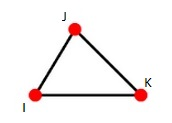
\includegraphics[width=0.25\textwidth]{./images/triangle_fe.jpg}
	\caption{Example a triangular finite element.}
	\label{fig:triangle_fe}
\end{figure}
        

    Note that for triangular elements, integrals can be performed in closed
form (without using quadrature).

\subsection{Cauchy Equilibrium
Equations}\label{cauchy-equilibrium-equations}


\begin{align*}
\frac{\partial \sigma_x}{\partial x} + \frac{\partial \tau_{xy}}{\partial y} +\frac{\partial \tau_{xz}}{\partial z} + X &= 0 \\
\frac{\partial \tau_{xy}}{\partial x} + \frac{\partial \sigma_y}{\partial y} +\frac{\partial \tau_{yz}}{\partial z} + Y &= 0 \\
\frac{\partial \tau_{xz}}{\partial x} + \frac{\partial \tau_{yz}}{\partial y} +\frac{\partial \sigma_z}{\partial z} + Z &= 0 \\
\end{align*}


    \subsection{Theorem of Virtual Work}\label{theorem-of-virtual-work}

\begin{quote}
A body is in equilibrium if and only if the virtual work of internal
forces is equal to the virtual work of the external forces for any
virtual displacement.
\end{quote}

\[
\underbrace{\delta L^i}_{\substack{\text{Work of}\\\text{internal forces}}} = \underbrace{\delta L^e}_{\substack{\text{Work of}\\\text{external forces}}}
\]

\[
\delta L^i = \iint_\Omega \underline{\sigma}^T \cdot \underline{\delta \epsilon}\, \mathrm{d}\Omega  
\]

\[
\delta L^e = \iint_\Omega \underline{X}^T \cdot \underline{\delta u}\, \mathrm{d}\Omega + \int_\Gamma \underline{t}^T \cdot \underline{\delta u}\, \mathrm{d}S
\]

\[
\underline{u}^e = 
\left( 
\begin{matrix}
u_e \\
v_e 
\end{matrix}
\right) 
= \underbrace{
\left( 
\begin{matrix}
\xi^e_i &       0 & \xi^e_j &       0 & \xi^e_k &       0 \\
      0 & \xi^e_i &       0 & \xi^e_j &       0 & \xi^e_k
\end{matrix}
\right)}_{\mathbf{N}^e}
\underbrace{\left( 
\begin{matrix}
u_i \\
v_i \\
u_j \\
v_j \\
u_k \\
v_k
\end{matrix}
\right)}_{\underline{u}^e_N}
\]

\[
\underline{\epsilon}^e = 
\left( 
\begin{matrix}
\frac{\partial}{\partial x} &                           0 \\
                          0 & \frac{\partial}{\partial y} \\
\frac{\partial}{\partial x} & \frac{\partial}{\partial y}
\end{matrix}
\right) 
\left( 
\begin{matrix}
\xi^e_i &       0 & \xi^e_j &       0 & \xi^e_k &       0 \\
      0 & \xi^e_i &       0 & \xi^e_j &       0 & \xi^e_k
\end{matrix}
\right)
\left( 
\begin{matrix}
u_i \\
v_i \\
u_j \\
v_j \\
u_k \\
v_k
\end{matrix}
\right)
\]

\[
\underline{\epsilon}^e = \underbrace{\frac{1}{2 \Delta^e}
\left( 
\begin{matrix}
b_i &   0 & b_j &   0 & b_k &   0 \\
  0 & c_i &   0 & c_j &   0 & c_k \\
b_i & c_i & b_j & c_j & b_k & c_k
\end{matrix}
\right)}_{\mathbf{B}^e}
\underline{u}^e_N
\]

\[
\underline{\epsilon}^e = \mathbf{B}^e \cdot \underline{u}^e_N
\]

We need to link deformation to stresses. Using linear elasticity and
focusing on the isotropic case the \textbf{constitutive equation}, in
matrix notation, is given by

\[
\underline{\sigma} = 
\left( 
\begin{matrix}
\sigma_x \\
\sigma_y \\
\tau_{xy}
\end{matrix}
\right) 
= \underbrace{\frac{E}{1 - \nu^2}
\left( 
\begin{matrix}
  1 & \nu &   0 \\
\nu &   1 &   0 \\
  0 &   0 & \frac{1-\nu}{2} 
\end{matrix}
\right)}_{\mathbf{D} = \text{Elastic Constitutive Matrix}}
\left( 
\begin{matrix}
\epsilon_x \\
\epsilon_y \\
\gamma_{xy}
\end{matrix}
\right)
\]

\[
\underline{\sigma} = \mathbf{D}^e \cdot \underline{\epsilon}
\]

    \[
\delta L^i = \iint_{\Delta^e} \underline{\sigma}^T \cdot \underline{\delta \epsilon}\, \mathrm{d}A = \iint_{\Delta^e} \underline{\delta \epsilon}^T \cdot \underline{\sigma} \, \mathrm{d}A
\]

\[
\underline{\delta \epsilon} = \mathbf{B}^e \cdot \delta \underline{u}^e_N
\]

\[
\underline{\sigma} = \mathbf{D}^e \cdot \underline{\epsilon} = \mathbf{D}^e \mathbf{B}^e \underline{u}^e_N
\]

\[
\delta L^i = (\underline{u}^e_N)^T \iint_{\Delta^e} (\mathbf{B}^e)^T \mathbf{D}^e \mathbf{B}^e \underline{u}^e_N \, \mathrm{d}A = (\underline{u}^e_N)^T \left[ \Delta^e (\mathbf{B}^e)^T \mathbf{D}^e \mathbf{B}^e \right] \underline{u}^e_N
\]

Now we need to compute \(\delta L^e\):


\begin{align*}
\delta L^e &= \iint_{\Delta^e} \underline{X}^T \mathbf{N}^e \delta \underline{u}^e_N\, \mathrm{d}A + \int_{\partial \Delta^e} \underline{t}^T \mathbf{N}^e \delta \underline{u}^e_N
\, \mathrm{d}S \\
&= (\delta \underline{u}^e_N)^T \underbrace{\left[ \iint_{\Delta^e} (\mathbf{N}^e)^T \underline{X} \, \mathrm{d}A + \int_{\partial \Delta^e} (\mathbf{N}^e)^T
\underline{t}\, \mathrm{d}S \right]}_{\underline{f}^e_N}
\end{align*}


By making the works equal, we get

\[
(\delta \underline{u}^e_N)^T \cdot \Delta^e \left[ (\mathbf{B}^e)^T \mathbf{D}^e \mathbf{B}^e \right] \underline{u}^e_N = (\delta \underline{u}^e_N)^T \cdot \underline{f}^e_N
\]

The linear system above is for each finite element and it results in a
global linear system as follows

\[
\mathbf{K} \vec{U} = \vec{F}
\]

where \(\mathbf{K}\) is the stiffness matrix, \(\vec{U}\) the unknowns
and \(\vec{F}\) the external forces.

    \section{Numerical
Implementation}\label{numerical-implementation}

Let's load our data. We'll work with two example cases: a small case and
a large case. The input data is rather large, hence it will be
configured in an external Python script (\texttt{fem\_data.py}). From
this script, we'll import the class \texttt{Setup} and the methods
\texttt{GetSetupLargeCase} and \texttt{GetSetupSmallCase}, as they will
configure our two examples. Of course that, from their own names, we can
infere that one corresponds to a large problem and the other one to a
small one.

The setup includes constants and variables such as the number of degrees
of freedom, the coordinates of each node, the number of elements and the
conectivity array, as well as the boundary conditions and properties of
our problem.

Some hipotesis that will be assumed are: 1. All elements have the same
number of nodes (triangles) 2. Properties are the same for all elements

    \begin{Verbatim}[commandchars=\\\{\}]
{\color{incolor}In [{\color{incolor}5}]:} \PY{k+kn}{from} \PY{n+nn}{fem\PYZus{}data} \PY{k+kn}{import} \PY{n}{Setup}\PY{p}{,} \PY{n}{GetSetupLargeCase}\PY{p}{,} \PY{n}{GetSetupSmallCase}
        \PY{n}{setup} \PY{o}{=} \PY{n}{Setup}\PY{p}{(}\PY{p}{)}
        \PY{c}{\PYZsh{}GetSetupSmallCase(setup)}
        \PY{n}{GetSetupLargeCase}\PY{p}{(}\PY{n}{setup}\PY{p}{)}
\end{Verbatim}

    \begin{Verbatim}[commandchars=\\\{\}]
{\color{incolor}In [{\color{incolor}6}]:} \PY{n}{number\PYZus{}of\PYZus{}dof}        \PY{o}{=} \PY{n}{setup}\PY{o}{.}\PY{n}{NumGL} \PY{c}{\PYZsh{} number of defrees of freedom}
        \PY{n}{number\PYZus{}of\PYZus{}nodes\PYZus{}el}   \PY{o}{=} \PY{n}{setup}\PY{o}{.}\PY{n}{NumNosEl}
        \PY{n}{number\PYZus{}of\PYZus{}nodes}      \PY{o}{=} \PY{n}{setup}\PY{o}{.}\PY{n}{NumNos}
        \PY{n}{coordinates}          \PY{o}{=} \PY{n}{setup}\PY{o}{.}\PY{n}{Coord}
        \PY{n}{number\PYZus{}of\PYZus{}elements}   \PY{o}{=} \PY{n}{setup}\PY{o}{.}\PY{n}{NumElem}
        \PY{n}{connectivity}         \PY{o}{=} \PY{n}{setup}\PY{o}{.}\PY{n}{Incid}
        \PY{n}{material\PYZus{}properties}  \PY{o}{=} \PY{n}{setup}\PY{o}{.}\PY{n}{PropMat}
        \PY{n}{geometric\PYZus{}properties} \PY{o}{=} \PY{n}{setup}\PY{o}{.}\PY{n}{PropGeo}
        \PY{n}{dirichlet\PYZus{}bc}         \PY{o}{=} \PY{n}{setup}\PY{o}{.}\PY{n}{CCDirichlet}
        \PY{n}{newmann\PYZus{}bc}           \PY{o}{=} \PY{n}{setup}\PY{o}{.}\PY{n}{CCNewmann}
        \PY{n}{body\PYZus{}force}           \PY{o}{=} \PY{n}{setup}\PY{o}{.}\PY{n}{Fcorpo}
\end{Verbatim}

    The method below is an auxiliary method that will plot the results that
we'll obtain from the FEM simulation, i.e, it will allow us to view the
initial and final conditions of our nodal variables.

    \begin{Verbatim}[commandchars=\\\{\}]
{\color{incolor}In [{\color{incolor}7}]:} \PY{k}{def} \PY{n+nf}{ViewMesh}\PY{p}{(}
            \PY{n}{coord}\PY{p}{,} 
            \PY{n}{connec}\PY{p}{,} 
            \PY{n}{hold}\PY{o}{=}\PY{n+nb+bp}{False}\PY{p}{,} 
            \PY{n}{show}\PY{o}{=}\PY{n+nb+bp}{True}\PY{p}{,} 
            \PY{n}{label}\PY{o}{=}\PY{l+s}{\PYZsq{}}\PY{l+s}{unknown}\PY{l+s}{\PYZsq{}}\PY{p}{,} 
            \PY{n}{node\PYZus{}color}\PY{o}{=}\PY{l+s}{\PYZsq{}}\PY{l+s}{r}\PY{l+s}{\PYZsq{}}\PY{p}{,} 
            \PY{n}{edge\PYZus{}color}\PY{o}{=}\PY{l+s}{\PYZsq{}}\PY{l+s}{k}\PY{l+s}{\PYZsq{}}
            \PY{p}{)}\PY{p}{:}
            
            \PY{k+kn}{import} \PY{n+nn}{networkx} \PY{k+kn}{as} \PY{n+nn}{nx}    
            \PY{n}{G} \PY{o}{=} \PY{n}{nx}\PY{o}{.}\PY{n}{Graph}\PY{p}{(}\PY{p}{)}
            
            \PY{n}{number\PYZus{}of\PYZus{}nodes} \PY{o}{=} \PY{n}{coord}\PY{o}{.}\PY{n}{shape}\PY{p}{[}\PY{l+m+mi}{0}\PY{p}{]}
            
            \PY{k}{for} \PY{n}{i}\PY{p}{,}\PY{n}{j}\PY{p}{,}\PY{n}{k} \PY{o+ow}{in} \PY{n}{connec}\PY{p}{:}        
                \PY{n}{G}\PY{o}{.}\PY{n}{add\PYZus{}edge}\PY{p}{(}\PY{n}{i}\PY{p}{,}\PY{n}{j}\PY{p}{)}
                \PY{n}{G}\PY{o}{.}\PY{n}{add\PYZus{}edge}\PY{p}{(}\PY{n}{i}\PY{p}{,}\PY{n}{k}\PY{p}{)}
                \PY{n}{G}\PY{o}{.}\PY{n}{add\PYZus{}edge}\PY{p}{(}\PY{n}{j}\PY{p}{,}\PY{n}{k}\PY{p}{)}
        
            \PY{n}{pos} \PY{o}{=} \PY{p}{\PYZob{}}\PY{p}{\PYZcb{}}
            \PY{k}{for} \PY{n}{n} \PY{o+ow}{in} \PY{n+nb}{xrange}\PY{p}{(}\PY{n}{number\PYZus{}of\PYZus{}nodes}\PY{p}{)}\PY{p}{:}
                \PY{n}{pos}\PY{p}{[}\PY{n}{n}\PY{p}{]} \PY{o}{=} \PY{n}{coord}\PY{p}{[}\PY{n}{n}\PY{p}{]}
            
            \PY{n}{node\PYZus{}size} \PY{o}{=} \PY{l+m+mi}{20} \PY{o}{+} \PY{p}{(}\PY{l+m+mi}{1000} \PY{o}{/} \PY{n}{number\PYZus{}of\PYZus{}nodes}\PY{p}{)}
            \PY{n}{nx}\PY{o}{.}\PY{n}{draw}\PY{p}{(}\PY{n}{G}\PY{p}{,} \PY{n}{pos}\PY{o}{=}\PY{n}{pos}\PY{p}{,} \PY{n}{hold}\PY{o}{=}\PY{n}{hold}\PY{p}{,} \PY{n}{node\PYZus{}color}\PY{o}{=}\PY{n}{node\PYZus{}color}\PY{p}{,} 
                    \PY{n}{label}\PY{o}{=}\PY{n}{label}\PY{p}{,} \PY{n}{edge\PYZus{}color}\PY{o}{=}\PY{n}{edge\PYZus{}color}\PY{p}{,} \PY{n}{node\PYZus{}size}\PY{o}{=}\PY{n}{node\PYZus{}size}\PY{p}{)}
            
            \PY{k}{if} \PY{n}{show}\PY{p}{:}
                \PY{n}{pyplot}\PY{o}{.}\PY{n}{show}\PY{p}{(}\PY{p}{)}
\end{Verbatim}

    \subsection{Element Stiffness Matrix}\label{element-stiffness-matrix}

The following method returns the \textbf{Stiffness Matrix} for the
linear triangle element in plane stress:

    \begin{Verbatim}[commandchars=\\\{\}]
{\color{incolor}In [{\color{incolor}8}]:} \PY{k}{def} \PY{n+nf}{KeT3\PYZus{}EPT}\PY{p}{(}\PY{n}{coord}\PY{p}{,} \PY{n}{mat\PYZus{}prop}\PY{p}{,} \PY{n}{geo\PYZus{}prop}\PY{p}{,} \PY{n}{body\PYZus{}force}\PY{p}{)}\PY{p}{:}
            \PY{l+s+sd}{\PYZsq{}\PYZsq{}\PYZsq{}}
        \PY{l+s+sd}{    Method that returns the Stiffness Matrix }
        \PY{l+s+sd}{    for the linear triangle element in plane }
        \PY{l+s+sd}{    stress.    }
        \PY{l+s+sd}{    }
        \PY{l+s+sd}{    \PYZsq{}\PYZsq{}\PYZsq{}}
            \PY{n}{Ex} \PY{o}{=} \PY{n}{mat\PYZus{}prop}\PY{p}{[}\PY{l+m+mi}{0}\PY{p}{]} \PY{c}{\PYZsh{} Young\PYZsq{}s modulus}
            \PY{n}{Nu} \PY{o}{=} \PY{n}{mat\PYZus{}prop}\PY{p}{[}\PY{l+m+mi}{1}\PY{p}{]} \PY{c}{\PYZsh{} Poisson\PYZsq{}s ratio}
            \PY{n}{t}  \PY{o}{=} \PY{n}{geo\PYZus{}prop}
        
            \PY{c}{\PYZsh{} Auxiliary functions}
            \PY{n}{ci} \PY{o}{=} \PY{o}{\PYZhy{}} \PY{n}{coord}\PY{p}{[}\PY{l+m+mi}{1}\PY{p}{,}\PY{l+m+mi}{0}\PY{p}{]} \PY{o}{+} \PY{n}{coord}\PY{p}{[}\PY{l+m+mi}{2}\PY{p}{,}\PY{l+m+mi}{0}\PY{p}{]}
            \PY{n}{cj} \PY{o}{=} \PY{o}{\PYZhy{}} \PY{n}{coord}\PY{p}{[}\PY{l+m+mi}{2}\PY{p}{,}\PY{l+m+mi}{0}\PY{p}{]} \PY{o}{+} \PY{n}{coord}\PY{p}{[}\PY{l+m+mi}{0}\PY{p}{,}\PY{l+m+mi}{0}\PY{p}{]}
            \PY{n}{ck} \PY{o}{=} \PY{o}{\PYZhy{}} \PY{n}{coord}\PY{p}{[}\PY{l+m+mi}{0}\PY{p}{,}\PY{l+m+mi}{0}\PY{p}{]} \PY{o}{+} \PY{n}{coord}\PY{p}{[}\PY{l+m+mi}{1}\PY{p}{,}\PY{l+m+mi}{0}\PY{p}{]}
        
            \PY{n}{bi} \PY{o}{=} \PY{o}{+} \PY{n}{coord}\PY{p}{[}\PY{l+m+mi}{1}\PY{p}{,}\PY{l+m+mi}{1}\PY{p}{]} \PY{o}{\PYZhy{}} \PY{n}{coord}\PY{p}{[}\PY{l+m+mi}{2}\PY{p}{,}\PY{l+m+mi}{1}\PY{p}{]}
            \PY{n}{bj} \PY{o}{=} \PY{o}{+} \PY{n}{coord}\PY{p}{[}\PY{l+m+mi}{2}\PY{p}{,}\PY{l+m+mi}{1}\PY{p}{]} \PY{o}{\PYZhy{}} \PY{n}{coord}\PY{p}{[}\PY{l+m+mi}{0}\PY{p}{,}\PY{l+m+mi}{1}\PY{p}{]}
            \PY{n}{bk} \PY{o}{=} \PY{o}{+} \PY{n}{coord}\PY{p}{[}\PY{l+m+mi}{0}\PY{p}{,}\PY{l+m+mi}{1}\PY{p}{]} \PY{o}{\PYZhy{}} \PY{n}{coord}\PY{p}{[}\PY{l+m+mi}{1}\PY{p}{,}\PY{l+m+mi}{1}\PY{p}{]}
        
            \PY{n}{d} \PY{o}{=} \PY{p}{(}\PY{n}{ck} \PY{o}{*} \PY{n}{bj} \PY{o}{\PYZhy{}} \PY{n}{cj} \PY{o}{*} \PY{n}{bk}\PY{p}{)}
            \PY{n}{area} \PY{o}{=} \PY{n}{d} \PY{o}{/} \PY{l+m+mi}{2}
        
            \PY{n}{B} \PY{o}{=} \PY{p}{(}\PY{l+m+mi}{1} \PY{o}{/} \PY{n}{d}\PY{p}{)} \PY{o}{*} \PY{n}{np}\PY{o}{.}\PY{n}{matrix}\PY{p}{(}\PY{p}{[}
                \PY{p}{[}\PY{n}{bi}\PY{p}{,}    \PY{l+m+mi}{0}\PY{p}{,}  \PY{n}{bj}\PY{p}{,}    \PY{l+m+mi}{0}\PY{p}{,}  \PY{n}{bk}\PY{p}{,}    \PY{l+m+mi}{0}\PY{p}{]}\PY{p}{,} 
                \PY{p}{[} \PY{l+m+mi}{0}\PY{p}{,}   \PY{n}{ci}\PY{p}{,}   \PY{l+m+mi}{0}\PY{p}{,}   \PY{n}{cj}\PY{p}{,}   \PY{l+m+mi}{0}\PY{p}{,}   \PY{n}{ck}\PY{p}{]}\PY{p}{,}
                \PY{p}{[}\PY{n}{ci}\PY{p}{,}   \PY{n}{bi}\PY{p}{,}  \PY{n}{cj}\PY{p}{,}   \PY{n}{bj}\PY{p}{,}  \PY{n}{ck}\PY{p}{,}   \PY{n}{bk}\PY{p}{]}
                \PY{p}{]}\PY{p}{)}
        
            \PY{n}{D} \PY{o}{=} \PY{n}{Ex} \PY{o}{/} \PY{p}{(}\PY{l+m+mi}{1} \PY{o}{\PYZhy{}} \PY{n}{Nu} \PY{o}{*}\PY{o}{*} \PY{l+m+mi}{2}\PY{p}{)} \PY{o}{*} \PY{n}{np}\PY{o}{.}\PY{n}{matrix}\PY{p}{(}\PY{p}{[}
                \PY{p}{[} \PY{l+m+mi}{1}\PY{p}{,}  \PY{n}{Nu}\PY{p}{,}            \PY{l+m+mi}{0}\PY{p}{]}\PY{p}{,}
                \PY{p}{[}\PY{n}{Nu}\PY{p}{,}   \PY{l+m+mi}{1}\PY{p}{,}            \PY{l+m+mi}{0}\PY{p}{]}\PY{p}{,}
                \PY{p}{[} \PY{l+m+mi}{0}\PY{p}{,}   \PY{l+m+mi}{0}\PY{p}{,} \PY{p}{(}\PY{l+m+mi}{1} \PY{o}{\PYZhy{}} \PY{n}{Nu}\PY{p}{)} \PY{o}{/} \PY{l+m+mi}{2}\PY{p}{]} 
                \PY{p}{]}\PY{p}{)}
        
            \PY{n}{Ke} \PY{o}{=} \PY{n}{B}\PY{o}{.}\PY{n}{T} \PY{o}{*} \PY{n}{D} \PY{o}{*} \PY{n}{B} \PY{o}{*} \PY{p}{(}\PY{n}{area} \PY{o}{*} \PY{n}{t}\PY{p}{)}
        
            \PY{n}{Fe1} \PY{o}{=} \PY{p}{(}\PY{n}{area} \PY{o}{*} \PY{n}{body\PYZus{}force}\PY{p}{[}\PY{l+m+mi}{0}\PY{p}{,}\PY{l+m+mi}{1}\PY{p}{]} \PY{o}{*} \PY{n}{t}
                \PY{o}{*}  \PY{n}{np}\PY{o}{.}\PY{n}{array}\PY{p}{(}\PY{p}{[}\PY{l+m+mi}{1}\PY{o}{/}\PY{l+m+mi}{3}\PY{p}{,} \PY{l+m+mf}{0.0}\PY{p}{,} \PY{l+m+mi}{1}\PY{o}{/}\PY{l+m+mi}{3}\PY{p}{,} \PY{l+m+mf}{0.0}\PY{p}{,} \PY{l+m+mi}{1}\PY{o}{/}\PY{l+m+mi}{3}\PY{p}{,} \PY{l+m+mf}{0.0}\PY{p}{]}\PY{p}{)}\PY{p}{)}
                
            \PY{n}{Fe2} \PY{o}{=} \PY{p}{(}\PY{n}{area} \PY{o}{*} \PY{n}{body\PYZus{}force}\PY{p}{[}\PY{l+m+mi}{1}\PY{p}{,}\PY{l+m+mi}{1}\PY{p}{]} \PY{o}{*} \PY{n}{t}
                \PY{o}{*}  \PY{n}{np}\PY{o}{.}\PY{n}{array}\PY{p}{(}\PY{p}{[}\PY{l+m+mf}{0.0}\PY{p}{,} \PY{l+m+mi}{1}\PY{o}{/}\PY{l+m+mi}{3}\PY{p}{,} \PY{l+m+mf}{0.0}\PY{p}{,} \PY{l+m+mi}{1}\PY{o}{/}\PY{l+m+mi}{3}\PY{p}{,} \PY{l+m+mf}{0.0}\PY{p}{,} \PY{l+m+mi}{1}\PY{o}{/}\PY{l+m+mi}{3}\PY{p}{]}\PY{p}{)}\PY{p}{)}
                
            \PY{n}{Fe} \PY{o}{=} \PY{n}{Fe1} \PY{o}{+} \PY{n}{Fe2}
            
            \PY{k}{return} \PY{n}{Ke}\PY{p}{,} \PY{n}{Fe}
\end{Verbatim}

    The code below will generate the matrix \texttt{ID} that enumerates each
equation (for \(x\) and \(y\) direction) to be solved.

    \begin{Verbatim}[commandchars=\\\{\}]
{\color{incolor}In [{\color{incolor}9}]:} \PY{n}{count} \PY{o}{=} \PY{l+m+mi}{0}
        \PY{n}{ID} \PY{o}{=} \PY{n}{np}\PY{o}{.}\PY{n}{zeros}\PY{p}{(}\PY{p}{(}\PY{n}{number\PYZus{}of\PYZus{}nodes}\PY{p}{,} \PY{n}{number\PYZus{}of\PYZus{}dof}\PY{p}{)}\PY{p}{)}
        \PY{k}{for} \PY{n}{n} \PY{o+ow}{in} \PY{n+nb}{xrange}\PY{p}{(}\PY{n}{number\PYZus{}of\PYZus{}nodes}\PY{p}{)}\PY{p}{:}
            \PY{k}{for} \PY{n}{dof} \PY{o+ow}{in} \PY{n+nb}{xrange}\PY{p}{(}\PY{n}{number\PYZus{}of\PYZus{}dof}\PY{p}{)}\PY{p}{:}
                \PY{n}{ID}\PY{p}{[}\PY{n}{n}\PY{p}{,}\PY{n}{dof}\PY{p}{]} \PY{o}{=} \PY{n}{count}
                \PY{n}{count} \PY{o}{+}\PY{o}{=} \PY{l+m+mi}{1}
        
        \PY{k}{assert} \PY{n}{count} \PY{o}{==} \PY{n}{number\PYZus{}of\PYZus{}dof} \PY{o}{*} \PY{n}{number\PYZus{}of\PYZus{}nodes}
\end{Verbatim}

    \subsection{Create the Linear System}\label{create-the-linear-system}

With the algorithm below, we'll build the global matrix \(\mathbf{K}\)
and global vector \(\vec{F}\).

    \begin{Verbatim}[commandchars=\\\{\}]
{\color{incolor}In [{\color{incolor}10}]:} \PY{n}{global\PYZus{}size} \PY{o}{=} \PY{n}{number\PYZus{}of\PYZus{}dof} \PY{o}{*} \PY{n}{number\PYZus{}of\PYZus{}nodes}
         
         \PY{n}{K} \PY{o}{=} \PY{n}{np}\PY{o}{.}\PY{n}{zeros}\PY{p}{(}\PY{p}{(}\PY{n}{global\PYZus{}size}\PY{p}{,}\PY{n}{global\PYZus{}size}\PY{p}{)}\PY{p}{)}
         \PY{n}{F} \PY{o}{=} \PY{n}{np}\PY{o}{.}\PY{n}{zeros}\PY{p}{(}\PY{p}{(}\PY{n}{global\PYZus{}size}\PY{p}{,}\PY{l+m+mi}{1}\PY{p}{)}\PY{p}{)}
         
         \PY{n}{size\PYZus{}el} \PY{o}{=} \PY{n}{number\PYZus{}of\PYZus{}dof} \PY{o}{*} \PY{n}{number\PYZus{}of\PYZus{}nodes\PYZus{}el}
         
         \PY{k}{for} \PY{n}{e} \PY{o+ow}{in} \PY{n+nb}{xrange}\PY{p}{(}\PY{n}{number\PYZus{}of\PYZus{}elements}\PY{p}{)}\PY{p}{:}
             
             \PY{c}{\PYZsh{} Builds element LM vector and element coordinates }
             \PY{c}{\PYZsh{} LM has the equations associated to element e}
             \PY{n}{LM} \PY{o}{=} \PY{n}{np}\PY{o}{.}\PY{n}{zeros}\PY{p}{(}\PY{n}{size\PYZus{}el}\PY{p}{)}
             \PY{n}{coord\PYZus{}el} \PY{o}{=} \PY{n}{np}\PY{o}{.}\PY{n}{zeros}\PY{p}{(}\PY{p}{(}\PY{n}{size\PYZus{}el}\PY{p}{,}\PY{l+m+mi}{2}\PY{p}{)}\PY{p}{)}
             
             \PY{n}{z} \PY{o}{=} \PY{l+m+mi}{0}
             \PY{k}{for} \PY{n}{j} \PY{o+ow}{in} \PY{n+nb}{xrange}\PY{p}{(}\PY{n}{number\PYZus{}of\PYZus{}nodes\PYZus{}el}\PY{p}{)}\PY{p}{:}
                 \PY{n}{J} \PY{o}{=} \PY{n}{connectivity}\PY{p}{[}\PY{n}{e}\PY{p}{,}\PY{n}{j}\PY{p}{]} \PY{c}{\PYZsh{} global node of element}
                 \PY{k}{for} \PY{n}{dof} \PY{o+ow}{in} \PY{n+nb}{xrange}\PY{p}{(}\PY{n}{number\PYZus{}of\PYZus{}dof}\PY{p}{)}\PY{p}{:}
                     \PY{n}{LM}\PY{p}{[}\PY{n}{z}\PY{p}{]} \PY{o}{=} \PY{n}{ID}\PY{p}{[}\PY{n}{J}\PY{p}{,}\PY{n}{dof}\PY{p}{]}
                     \PY{n}{z} \PY{o}{+}\PY{o}{=} \PY{l+m+mi}{1}      
         
                 \PY{k}{for} \PY{n}{k} \PY{o+ow}{in} \PY{n+nb}{xrange}\PY{p}{(}\PY{l+m+mi}{2}\PY{p}{)}\PY{p}{:}
                     \PY{n}{coord\PYZus{}el}\PY{p}{[}\PY{n}{j}\PY{p}{,}\PY{n}{k}\PY{p}{]} \PY{o}{=} \PY{n}{coordinates}\PY{p}{[}\PY{n}{J}\PY{p}{,}\PY{n}{k}\PY{p}{]}
         
             \PY{c}{\PYZsh{} Calls method that calculates element}
             \PY{c}{\PYZsh{} matrix Ke and element load vector Fe}
             \PY{n}{Ke}\PY{p}{,} \PY{n}{Fe} \PY{o}{=} \PY{n}{KeT3\PYZus{}EPT}\PY{p}{(}
                 \PY{n}{coord\PYZus{}el}\PY{p}{,} 
                 \PY{n}{material\PYZus{}properties}\PY{p}{,} 
                 \PY{n}{geometric\PYZus{}properties}\PY{p}{,}
                 \PY{n}{body\PYZus{}force}
                 \PY{p}{)}
            
             \PY{k}{for} \PY{n}{i} \PY{o+ow}{in} \PY{n+nb}{xrange}\PY{p}{(}\PY{n}{size\PYZus{}el}\PY{p}{)}\PY{p}{:}
                 \PY{n}{I} \PY{o}{=} \PY{n}{LM}\PY{p}{[}\PY{n}{i}\PY{p}{]}
                 \PY{k}{for} \PY{n}{j} \PY{o+ow}{in} \PY{n+nb}{xrange}\PY{p}{(}\PY{n}{size\PYZus{}el}\PY{p}{)}\PY{p}{:}
                     \PY{n}{J} \PY{o}{=} \PY{n}{LM}\PY{p}{[}\PY{n}{j}\PY{p}{]}  
                     \PY{c}{\PYZsh{} Adds element matrix Ke to global matrix K}
                     \PY{n}{K}\PY{p}{[}\PY{n}{I}\PY{p}{,}\PY{n}{J}\PY{p}{]} \PY{o}{+}\PY{o}{=} \PY{n}{Ke}\PY{p}{[}\PY{n}{i}\PY{p}{,}\PY{n}{j}\PY{p}{]}
                 \PY{c}{\PYZsh{} Adds load vector Fe in F        }
                 \PY{n}{F}\PY{p}{[}\PY{n}{I}\PY{p}{]} \PY{o}{=} \PY{n}{F}\PY{p}{[}\PY{n}{I}\PY{p}{]} \PY{o}{+} \PY{n}{Fe}\PY{p}{[}\PY{n}{i}\PY{p}{]} 
\end{Verbatim}

    \subsection{Boundary Conditions}\label{boundary-conditions}

Now we'll introduce the Newmann boundary condition to the load vector
\(\vec{F}\):

    \begin{Verbatim}[commandchars=\\\{\}]
{\color{incolor}In [{\color{incolor}11}]:} \PY{k}{for} \PY{n}{node}\PY{p}{,} \PY{n}{dof}\PY{p}{,} \PY{n}{value} \PY{o+ow}{in} \PY{n}{newmann\PYZus{}bc}\PY{p}{:}
             \PY{n}{eq}    \PY{o}{=} \PY{n}{ID}\PY{p}{[}\PY{n}{node}\PY{p}{,}\PY{n}{dof}\PY{p}{]}
             \PY{n}{F}\PY{p}{[}\PY{n}{eq}\PY{p}{]} \PY{o}{=} \PY{n}{F}\PY{p}{[}\PY{n}{eq}\PY{p}{]} \PY{o}{+} \PY{n}{value}
\end{Verbatim}

    For the Dirichlet boundary conditions, the unkown has a prescribed
value. In this case, we set the line of the matrix associated to that
unknown to zero with the value one in the diagonal. Moreover, we
subtract the product of the column of the matrix that corresponds to the
precribed unknown time the prescribed value from the independent vector
and make that column equal to zero (the size of the final linear system
could be reduced).

    \begin{Verbatim}[commandchars=\\\{\}]
{\color{incolor}In [{\color{incolor}12}]:} \PY{k}{for} \PY{n}{node}\PY{p}{,} \PY{n}{dof}\PY{p}{,} \PY{n}{value} \PY{o+ow}{in} \PY{n}{dirichlet\PYZus{}bc}\PY{p}{:}    
             \PY{n}{eq} \PY{o}{=} \PY{n}{ID}\PY{p}{[}\PY{n}{node}\PY{p}{,}\PY{n}{dof}\PY{p}{]}
             \PY{n}{F}\PY{p}{[}\PY{p}{:}\PY{p}{,} \PY{l+m+mi}{0}\PY{p}{]} \PY{o}{=} \PY{n}{F}\PY{p}{[}\PY{p}{:}\PY{p}{,} \PY{l+m+mi}{0}\PY{p}{]} \PY{o}{\PYZhy{}} \PY{n}{value} \PY{o}{*} \PY{n}{K}\PY{p}{[}\PY{p}{:}\PY{p}{,} \PY{n}{eq}\PY{p}{]}
             
             \PY{c}{\PYZsh{} zeros the whole line and column}
             \PY{c}{\PYZsh{} associated to eq, except the}
             \PY{c}{\PYZsh{} diagonal that is equal to 1.0}
             \PY{n}{K}\PY{p}{[}\PY{n}{eq}\PY{p}{,}\PY{p}{:}\PY{p}{]} \PY{o}{=} \PY{l+m+mf}{0.0}
             \PY{n}{K}\PY{p}{[}\PY{p}{:}\PY{p}{,}\PY{n}{eq}\PY{p}{]} \PY{o}{=} \PY{l+m+mf}{0.0}
             \PY{n}{K}\PY{p}{[}\PY{n}{eq}\PY{p}{,}\PY{n}{eq}\PY{p}{]} \PY{o}{=} \PY{l+m+mf}{1.0}
             \PY{n}{F}\PY{p}{[}\PY{n}{eq}\PY{p}{]} \PY{o}{=} \PY{n}{value}
\end{Verbatim}

    \subsection{Solve Linear System}\label{solve-linear-system}

With the global linear system complete with the boudnary condtiions, we
can move on to solve the resulting linear system
\(\mathbf{K} \vec{U} = \vec{F}\) for the static problem:

    \begin{Verbatim}[commandchars=\\\{\}]
{\color{incolor}In [{\color{incolor}13}]:} \PY{n}{U} \PY{o}{=} \PY{n}{np}\PY{o}{.}\PY{n}{linalg}\PY{o}{.}\PY{n}{solve}\PY{p}{(}\PY{n}{K}\PY{p}{,} \PY{n}{F}\PY{p}{)}
\end{Verbatim}

    With the resulting deformation vector \(\vec{U}\) we can generate the
deformed coordinates for the elements:

    \begin{Verbatim}[commandchars=\\\{\}]
{\color{incolor}In [{\color{incolor}14}]:} \PY{n}{coord\PYZus{}def} \PY{o}{=} \PY{n}{np}\PY{o}{.}\PY{n}{zeros}\PY{p}{(}\PY{p}{(}\PY{n}{number\PYZus{}of\PYZus{}nodes}\PY{p}{,} \PY{l+m+mi}{2}\PY{p}{)}\PY{p}{)}
         \PY{n}{Uf} \PY{o}{=} \PY{n}{np}\PY{o}{.}\PY{n}{zeros}\PY{p}{(}\PY{p}{(}\PY{n}{number\PYZus{}of\PYZus{}nodes}\PY{p}{,} \PY{n}{number\PYZus{}of\PYZus{}dof}\PY{p}{)}\PY{p}{)}
         
         \PY{n}{b} \PY{o}{=} \PY{l+m+mi}{0}
         \PY{k}{for} \PY{n}{n} \PY{o+ow}{in} \PY{n+nb}{xrange}\PY{p}{(}\PY{n}{number\PYZus{}of\PYZus{}nodes}\PY{p}{)}\PY{p}{:}
             \PY{k}{for} \PY{n}{dof} \PY{o+ow}{in} \PY{n+nb}{xrange}\PY{p}{(}\PY{n}{number\PYZus{}of\PYZus{}dof}\PY{p}{)}\PY{p}{:}
                 \PY{n}{Uf}\PY{p}{[}\PY{n}{n}\PY{p}{,}\PY{n}{dof}\PY{p}{]} \PY{o}{=} \PY{n}{U}\PY{p}{[}\PY{n}{b}\PY{p}{]}
                 \PY{n}{b} \PY{o}{+}\PY{o}{=} \PY{l+m+mi}{1}
         
         \PY{c}{\PYZsh{} Amplifying factor for vizualization purposes}
         \PY{n}{factor} \PY{o}{=} \PY{l+m+mi}{100}
         
         \PY{k}{for} \PY{n}{i} \PY{o+ow}{in} \PY{n+nb}{xrange}\PY{p}{(}\PY{n}{number\PYZus{}of\PYZus{}nodes}\PY{p}{)}\PY{p}{:}
             \PY{n}{coord\PYZus{}def}\PY{p}{[}\PY{n}{i}\PY{p}{,}\PY{l+m+mi}{0}\PY{p}{]} \PY{o}{=} \PY{n}{coordinates}\PY{p}{[}\PY{n}{i}\PY{p}{,}\PY{l+m+mi}{0}\PY{p}{]} \PY{o}{+} \PY{n}{factor} \PY{o}{*} \PY{n}{Uf}\PY{p}{[}\PY{n}{i}\PY{p}{,}\PY{l+m+mi}{0}\PY{p}{]}
             \PY{n}{coord\PYZus{}def}\PY{p}{[}\PY{n}{i}\PY{p}{,}\PY{l+m+mi}{1}\PY{p}{]} \PY{o}{=} \PY{n}{coordinates}\PY{p}{[}\PY{n}{i}\PY{p}{,}\PY{l+m+mi}{1}\PY{p}{]} \PY{o}{+} \PY{n}{factor} \PY{o}{*} \PY{n}{Uf}\PY{p}{[}\PY{n}{i}\PY{p}{,}\PY{l+m+mi}{1}\PY{p}{]}
\end{Verbatim}

    \subsection{View results}\label{view-results}

With our \texttt{ViewMesh} method defined previously, we can view the
results from the linear system:

    \begin{Verbatim}[commandchars=\\\{\}]
{\color{incolor}In [{\color{incolor}15}]:} \PY{n}{f} \PY{o}{=} \PY{n}{plt}\PY{o}{.}\PY{n}{figure}\PY{p}{(}\PY{p}{)}
         \PY{n}{ViewMesh}\PY{p}{(}\PY{n}{coord\PYZus{}def}\PY{p}{,} \PY{n}{connectivity}\PY{p}{,} \PY{n}{hold}\PY{o}{=}\PY{n+nb+bp}{True}\PY{p}{,} \PY{n}{show}\PY{o}{=}\PY{n+nb+bp}{False}\PY{p}{,} 
                  \PY{n}{label}\PY{o}{=}\PY{l+s}{\PYZsq{}}\PY{l+s}{Deformed}\PY{l+s}{\PYZsq{}}\PY{p}{,} \PY{n}{node\PYZus{}color}\PY{o}{=}\PY{l+s}{\PYZsq{}}\PY{l+s}{r}\PY{l+s}{\PYZsq{}}\PY{p}{,} \PY{n}{edge\PYZus{}color}\PY{o}{=}\PY{l+s}{\PYZsq{}}\PY{l+s}{k}\PY{l+s}{\PYZsq{}}\PY{p}{)}
         \PY{n}{ViewMesh}\PY{p}{(}\PY{n}{coordinates}\PY{p}{,} \PY{n}{connectivity}\PY{p}{,} \PY{n}{hold}\PY{o}{=}\PY{n+nb+bp}{True}\PY{p}{,} \PY{n}{show}\PY{o}{=}\PY{n+nb+bp}{False}\PY{p}{,} 
                  \PY{n}{label}\PY{o}{=}\PY{l+s}{\PYZsq{}}\PY{l+s}{Original}\PY{l+s}{\PYZsq{}}\PY{p}{,} \PY{n}{node\PYZus{}color}\PY{o}{=}\PY{l+s}{\PYZsq{}}\PY{l+s}{b}\PY{l+s}{\PYZsq{}}\PY{p}{,} \PY{n}{edge\PYZus{}color}\PY{o}{=}\PY{l+s}{\PYZsq{}}\PY{l+s}{0.5}\PY{l+s}{\PYZsq{}}\PY{p}{)}
         
         \PY{n}{ax} \PY{o}{=} \PY{n}{plt}\PY{o}{.}\PY{n}{gca}\PY{p}{(}\PY{p}{)}
         \PY{n}{handles}\PY{p}{,} \PY{n}{labels} \PY{o}{=} \PY{n}{ax}\PY{o}{.}\PY{n}{get\PYZus{}legend\PYZus{}handles\PYZus{}labels}\PY{p}{(}\PY{p}{)}
         
         \PY{n}{plt}\PY{o}{.}\PY{n}{legend}\PY{p}{(}\PY{n}{handles}\PY{o}{=}\PY{p}{[}\PY{n}{handles}\PY{p}{[}\PY{l+m+mi}{0}\PY{p}{]}\PY{p}{,} \PY{n}{handles}\PY{p}{[}\PY{l+m+mi}{2}\PY{p}{]}\PY{p}{]}\PY{p}{,}\PY{n}{bbox\PYZus{}to\PYZus{}anchor}\PY{o}{=}\PY{p}{(}\PY{l+m+mf}{0.8}\PY{p}{,} \PY{l+m+mi}{1}\PY{p}{)}\PY{p}{,}
                    \PY{n}{bbox\PYZus{}transform}\PY{o}{=}\PY{n}{plt}\PY{o}{.}\PY{n}{gcf}\PY{p}{(}\PY{p}{)}\PY{o}{.}\PY{n}{transFigure}\PY{p}{)}
         
         \PY{n}{f}\PY{o}{.}\PY{n}{set\PYZus{}size\PYZus{}inches}\PY{p}{(}\PY{l+m+mi}{10}\PY{p}{,}\PY{l+m+mi}{8}\PY{p}{)}
         \PY{n}{plt}\PY{o}{.}\PY{n}{show}\PY{p}{(}\PY{p}{)}
\end{Verbatim}

    \begin{center}
    \adjustimage{max size={0.9\linewidth}{0.9\paperheight}}{fem-python_files/fem-python_32_0.png}
    \end{center}
    { \hspace*{\fill} \\}
    
    \subsection{Element Stress}\label{element-stress}

The following method returns the \textbf{stress} for the linear triangle
element in plane stress. The principal stress are obtained by
calculating the eigenvalues of the element stress matrix.

    \begin{Verbatim}[commandchars=\\\{\}]
{\color{incolor}In [{\color{incolor}16}]:} \PY{k}{def} \PY{n+nf}{StressT3\PYZus{}EPT}\PY{p}{(}\PY{n}{coord}\PY{p}{,} \PY{n}{UEl}\PY{p}{,} \PY{n}{mat\PYZus{}prop}\PY{p}{,} \PY{n}{geo\PYZus{}prop}\PY{p}{)}\PY{p}{:}
             \PY{l+s+sd}{\PYZsq{}\PYZsq{}\PYZsq{}}
         \PY{l+s+sd}{    Method that returns the Stress for the }
         \PY{l+s+sd}{    linear triangle element in plane stress.    }
         \PY{l+s+sd}{    }
         \PY{l+s+sd}{    \PYZsq{}\PYZsq{}\PYZsq{}}    
             \PY{n}{Ex} \PY{o}{=} \PY{n}{mat\PYZus{}prop}\PY{p}{[}\PY{l+m+mi}{0}\PY{p}{]} \PY{c}{\PYZsh{} Young\PYZsq{}s modulus}
             \PY{n}{Nu} \PY{o}{=} \PY{n}{mat\PYZus{}prop}\PY{p}{[}\PY{l+m+mi}{1}\PY{p}{]} \PY{c}{\PYZsh{} Poisson\PYZsq{}s ratio}
             \PY{n}{t}  \PY{o}{=} \PY{n}{geo\PYZus{}prop}
         
             \PY{c}{\PYZsh{} Auxiliary functions}
             \PY{n}{ci} \PY{o}{=} \PY{o}{\PYZhy{}} \PY{n}{coord}\PY{p}{[}\PY{l+m+mi}{1}\PY{p}{,}\PY{l+m+mi}{0}\PY{p}{]} \PY{o}{+} \PY{n}{coord}\PY{p}{[}\PY{l+m+mi}{2}\PY{p}{,}\PY{l+m+mi}{0}\PY{p}{]}
             \PY{n}{cj} \PY{o}{=} \PY{o}{\PYZhy{}} \PY{n}{coord}\PY{p}{[}\PY{l+m+mi}{2}\PY{p}{,}\PY{l+m+mi}{0}\PY{p}{]} \PY{o}{+} \PY{n}{coord}\PY{p}{[}\PY{l+m+mi}{0}\PY{p}{,}\PY{l+m+mi}{0}\PY{p}{]}
             \PY{n}{ck} \PY{o}{=} \PY{o}{\PYZhy{}} \PY{n}{coord}\PY{p}{[}\PY{l+m+mi}{0}\PY{p}{,}\PY{l+m+mi}{0}\PY{p}{]} \PY{o}{+} \PY{n}{coord}\PY{p}{[}\PY{l+m+mi}{1}\PY{p}{,}\PY{l+m+mi}{0}\PY{p}{]}
         
             \PY{n}{bi} \PY{o}{=} \PY{o}{+} \PY{n}{coord}\PY{p}{[}\PY{l+m+mi}{1}\PY{p}{,}\PY{l+m+mi}{1}\PY{p}{]} \PY{o}{\PYZhy{}} \PY{n}{coord}\PY{p}{[}\PY{l+m+mi}{2}\PY{p}{,}\PY{l+m+mi}{1}\PY{p}{]}
             \PY{n}{bj} \PY{o}{=} \PY{o}{+} \PY{n}{coord}\PY{p}{[}\PY{l+m+mi}{2}\PY{p}{,}\PY{l+m+mi}{1}\PY{p}{]} \PY{o}{\PYZhy{}} \PY{n}{coord}\PY{p}{[}\PY{l+m+mi}{0}\PY{p}{,}\PY{l+m+mi}{1}\PY{p}{]}
             \PY{n}{bk} \PY{o}{=} \PY{o}{+} \PY{n}{coord}\PY{p}{[}\PY{l+m+mi}{0}\PY{p}{,}\PY{l+m+mi}{1}\PY{p}{]} \PY{o}{\PYZhy{}} \PY{n}{coord}\PY{p}{[}\PY{l+m+mi}{1}\PY{p}{,}\PY{l+m+mi}{1}\PY{p}{]}
         
             \PY{n}{d} \PY{o}{=} \PY{p}{(}\PY{n}{ck} \PY{o}{*} \PY{n}{bj} \PY{o}{\PYZhy{}} \PY{n}{cj} \PY{o}{*} \PY{n}{bk}\PY{p}{)}
             \PY{n}{area} \PY{o}{=} \PY{n}{d} \PY{o}{/} \PY{l+m+mi}{2}
         
             \PY{n}{B} \PY{o}{=} \PY{p}{(}\PY{l+m+mi}{1} \PY{o}{/} \PY{n}{d}\PY{p}{)} \PY{o}{*} \PY{n}{np}\PY{o}{.}\PY{n}{matrix}\PY{p}{(}\PY{p}{[}
                 \PY{p}{[}\PY{n}{bi}\PY{p}{,}    \PY{l+m+mi}{0}\PY{p}{,}  \PY{n}{bj}\PY{p}{,}    \PY{l+m+mi}{0}\PY{p}{,}  \PY{n}{bk}\PY{p}{,}    \PY{l+m+mi}{0}\PY{p}{]}\PY{p}{,} 
                 \PY{p}{[} \PY{l+m+mi}{0}\PY{p}{,}   \PY{n}{ci}\PY{p}{,}   \PY{l+m+mi}{0}\PY{p}{,}   \PY{n}{cj}\PY{p}{,}   \PY{l+m+mi}{0}\PY{p}{,}   \PY{n}{ck}\PY{p}{]}\PY{p}{,}
                 \PY{p}{[}\PY{n}{ci}\PY{p}{,}   \PY{n}{bi}\PY{p}{,}  \PY{n}{cj}\PY{p}{,}   \PY{n}{bj}\PY{p}{,}  \PY{n}{ck}\PY{p}{,}   \PY{n}{bk}\PY{p}{]}
                 \PY{p}{]}\PY{p}{)}
         
             \PY{n}{D} \PY{o}{=} \PY{n}{Ex} \PY{o}{/} \PY{p}{(}\PY{l+m+mi}{1} \PY{o}{\PYZhy{}} \PY{n}{Nu} \PY{o}{*}\PY{o}{*} \PY{l+m+mi}{2}\PY{p}{)} \PY{o}{*} \PY{n}{np}\PY{o}{.}\PY{n}{matrix}\PY{p}{(}\PY{p}{[}
                 \PY{p}{[} \PY{l+m+mi}{1}\PY{p}{,}  \PY{n}{Nu}\PY{p}{,}            \PY{l+m+mi}{0}\PY{p}{]}\PY{p}{,}
                 \PY{p}{[}\PY{n}{Nu}\PY{p}{,}   \PY{l+m+mi}{1}\PY{p}{,}            \PY{l+m+mi}{0}\PY{p}{]}\PY{p}{,}
                 \PY{p}{[} \PY{l+m+mi}{0}\PY{p}{,}   \PY{l+m+mi}{0}\PY{p}{,} \PY{p}{(}\PY{l+m+mi}{1} \PY{o}{\PYZhy{}} \PY{n}{Nu}\PY{p}{)} \PY{o}{/} \PY{l+m+mi}{2}\PY{p}{]} 
                 \PY{p}{]}\PY{p}{)}   
         
             \PY{n}{StressE} \PY{o}{=} \PY{n}{D} \PY{o}{*} \PY{n}{B} \PY{o}{*} \PY{n}{UEl}\PY{o}{.}\PY{n}{T}
                
             \PY{c}{\PYZsh{} Create 2D stress matrix}
             \PY{n}{S} \PY{o}{=} \PY{n}{np}\PY{o}{.}\PY{n}{zeros}\PY{p}{(}\PY{p}{(}\PY{n}{number\PYZus{}of\PYZus{}dof}\PY{p}{,} \PY{n}{number\PYZus{}of\PYZus{}dof}\PY{p}{)}\PY{p}{)}
             \PY{n}{S}\PY{p}{[}\PY{l+m+mi}{0}\PY{p}{,}\PY{l+m+mi}{0}\PY{p}{]} \PY{o}{=} \PY{n}{StressE}\PY{p}{[}\PY{l+m+mi}{0}\PY{p}{]}
             \PY{n}{S}\PY{p}{[}\PY{l+m+mi}{1}\PY{p}{,}\PY{l+m+mi}{1}\PY{p}{]} \PY{o}{=} \PY{n}{StressE}\PY{p}{[}\PY{l+m+mi}{1}\PY{p}{]}
             \PY{n}{S}\PY{p}{[}\PY{l+m+mi}{1}\PY{p}{,}\PY{l+m+mi}{0}\PY{p}{]} \PY{o}{=} \PY{n}{S}\PY{p}{[}\PY{l+m+mi}{0}\PY{p}{,}\PY{l+m+mi}{1}\PY{p}{]} \PY{o}{=} \PY{n}{StressE}\PY{p}{[}\PY{l+m+mi}{2}\PY{p}{]}
             
             \PY{c}{\PYZsh{} Stress in z direction is ZERO }
             \PY{c}{\PYZsh{} under plane stress conditions}
             \PY{n}{StressE} \PY{o}{=} \PY{n}{np}\PY{o}{.}\PY{n}{append}\PY{p}{(}\PY{n}{StressE}\PY{p}{,} \PY{p}{[}\PY{p}{[}\PY{l+m+mi}{0}\PY{p}{]}\PY{p}{]}\PY{p}{,} \PY{n}{axis}\PY{o}{=}\PY{l+m+mi}{0}\PY{p}{)}
             
             \PY{c}{\PYZsh{} Calculate principal stresses by }
             \PY{c}{\PYZsh{} finding the eigenvalues of S }
             \PY{n}{w}\PY{p}{,} \PY{n}{v} \PY{o}{=} \PY{n}{np}\PY{o}{.}\PY{n}{linalg}\PY{o}{.}\PY{n}{eig}\PY{p}{(}\PY{n}{S}\PY{p}{)}
             \PY{n}{s1}\PY{p}{,} \PY{n}{s2} \PY{o}{=} \PY{n}{w}
             
             \PY{c}{\PYZsh{} Von Mises Stress}
             \PY{n}{SVME} \PY{o}{=} \PY{n}{np}\PY{o}{.}\PY{n}{sqrt}\PY{p}{(}\PY{n}{s1} \PY{o}{*}\PY{o}{*} \PY{l+m+mi}{2} \PY{o}{\PYZhy{}} \PY{n}{s1}\PY{o}{*}\PY{n}{s2} \PY{o}{+} \PY{n}{s2} \PY{o}{*}\PY{o}{*} \PY{l+m+mi}{2}\PY{p}{)}
         
             \PY{c}{\PYZsh{} Tresca Stress}
             \PY{n}{STRE} \PY{o}{=} \PY{l+m+mf}{0.5} \PY{o}{*} \PY{n}{np}\PY{o}{.}\PY{n}{abs}\PY{p}{(}\PY{n}{s1} \PY{o}{\PYZhy{}} \PY{n}{s2}\PY{p}{)}
         
             \PY{k}{return} \PY{n}{StressE}\PY{p}{,} \PY{n}{SVME}\PY{p}{,} \PY{n}{STRE}
\end{Verbatim}

    \subsection{Stress calculation}\label{stress-calculation}

Calulates the stress and performs averaging.

    \begin{Verbatim}[commandchars=\\\{\}]
{\color{incolor}In [{\color{incolor}17}]:} \PY{n}{count} \PY{o}{=} \PY{n}{np}\PY{o}{.}\PY{n}{zeros}\PY{p}{(}\PY{n}{number\PYZus{}of\PYZus{}nodes}\PY{p}{)}
         \PY{n}{Sx}   \PY{o}{=} \PY{n}{np}\PY{o}{.}\PY{n}{zeros}\PY{p}{(}\PY{n}{number\PYZus{}of\PYZus{}nodes}\PY{p}{)}
         \PY{n}{Sy}   \PY{o}{=} \PY{n}{np}\PY{o}{.}\PY{n}{zeros}\PY{p}{(}\PY{n}{number\PYZus{}of\PYZus{}nodes}\PY{p}{)}
         \PY{n}{Sxy}  \PY{o}{=} \PY{n}{np}\PY{o}{.}\PY{n}{zeros}\PY{p}{(}\PY{n}{number\PYZus{}of\PYZus{}nodes}\PY{p}{)}
         \PY{n}{Sz}   \PY{o}{=} \PY{n}{np}\PY{o}{.}\PY{n}{zeros}\PY{p}{(}\PY{n}{number\PYZus{}of\PYZus{}nodes}\PY{p}{)}
         \PY{n}{SVM}  \PY{o}{=} \PY{n}{np}\PY{o}{.}\PY{n}{zeros}\PY{p}{(}\PY{n}{number\PYZus{}of\PYZus{}nodes}\PY{p}{)}
         \PY{n}{STR}  \PY{o}{=} \PY{n}{np}\PY{o}{.}\PY{n}{zeros}\PY{p}{(}\PY{n}{number\PYZus{}of\PYZus{}nodes}\PY{p}{)}
         
         \PY{k}{for} \PY{n}{e} \PY{o+ow}{in} \PY{n+nb}{xrange}\PY{p}{(}\PY{n}{number\PYZus{}of\PYZus{}elements}\PY{p}{)}\PY{p}{:}
             
             \PY{c}{\PYZsh{} Builds element LM vector and element coordinates }
             \PY{c}{\PYZsh{} and element displacement}
             \PY{n}{LM} \PY{o}{=} \PY{n}{np}\PY{o}{.}\PY{n}{zeros}\PY{p}{(}\PY{n}{size\PYZus{}el}\PY{p}{)}
             \PY{n}{UEl} \PY{o}{=} \PY{n}{np}\PY{o}{.}\PY{n}{zeros}\PY{p}{(}\PY{n}{size\PYZus{}el}\PY{p}{)}    
             \PY{n}{coord\PYZus{}el} \PY{o}{=} \PY{n}{np}\PY{o}{.}\PY{n}{zeros}\PY{p}{(}\PY{p}{(}\PY{n}{size\PYZus{}el}\PY{p}{,}\PY{l+m+mi}{2}\PY{p}{)}\PY{p}{)}
             
             \PY{n}{z} \PY{o}{=} \PY{l+m+mi}{0}
             \PY{k}{for} \PY{n}{j} \PY{o+ow}{in} \PY{n+nb}{xrange}\PY{p}{(}\PY{n}{number\PYZus{}of\PYZus{}nodes\PYZus{}el}\PY{p}{)}\PY{p}{:}
                 \PY{n}{J} \PY{o}{=} \PY{n}{connectivity}\PY{p}{[}\PY{n}{e}\PY{p}{,}\PY{n}{j}\PY{p}{]}
                 \PY{k}{for} \PY{n}{i} \PY{o+ow}{in} \PY{n+nb}{xrange}\PY{p}{(}\PY{n}{number\PYZus{}of\PYZus{}dof}\PY{p}{)}\PY{p}{:}
                     \PY{n}{LM}\PY{p}{[}\PY{n}{z}\PY{p}{]}  \PY{o}{=} \PY{n}{ID}\PY{p}{[}\PY{n}{J}\PY{p}{,}\PY{n}{i}\PY{p}{]}
                     \PY{n}{UEl}\PY{p}{[}\PY{n}{z}\PY{p}{]} \PY{o}{=} \PY{n}{Uf}\PY{p}{[}\PY{n}{J}\PY{p}{,}\PY{n}{i}\PY{p}{]}
                     \PY{n}{z} \PY{o}{+}\PY{o}{=} \PY{l+m+mi}{1}
               
                 \PY{k}{for} \PY{n}{k} \PY{o+ow}{in} \PY{n+nb}{xrange}\PY{p}{(}\PY{l+m+mi}{2}\PY{p}{)}\PY{p}{:}
                     \PY{n}{coord\PYZus{}el}\PY{p}{[}\PY{n}{j}\PY{p}{,}\PY{n}{k}\PY{p}{]} \PY{o}{=} \PY{n}{coordinates}\PY{p}{[}\PY{n}{J}\PY{p}{,}\PY{n}{k}\PY{p}{]}
           
             \PY{c}{\PYZsh{} Calls method that calculates element}
             \PY{c}{\PYZsh{} stress StressE, von Mises stress SVME}
             \PY{c}{\PYZsh{} and Tresca stress STRE}
             \PY{n}{StressE}\PY{p}{,} \PY{n}{SVME}\PY{p}{,} \PY{n}{STRE} \PY{o}{=} \PY{n}{StressT3\PYZus{}EPT}\PY{p}{(}
                 \PY{n}{coord\PYZus{}el}\PY{p}{,} 
                 \PY{n}{np}\PY{o}{.}\PY{n}{matrix}\PY{p}{(}\PY{n}{UEl}\PY{p}{)}\PY{p}{,} 
                 \PY{n}{material\PYZus{}properties}\PY{p}{,} 
                 \PY{n}{geometric\PYZus{}properties}
                 \PY{p}{)} 
            
             \PY{n}{i}\PY{p}{,} \PY{n}{j}\PY{p}{,} \PY{n}{k} \PY{o}{=} \PY{n}{connectivity}\PY{p}{[}\PY{n}{e}\PY{p}{]}
         
             \PY{n}{Sx}\PY{p}{[}\PY{n}{i}\PY{p}{]} \PY{o}{=} \PY{n}{Sx}\PY{p}{[}\PY{n}{i}\PY{p}{]} \PY{o}{+} \PY{n}{StressE}\PY{p}{[}\PY{l+m+mi}{0}\PY{p}{]}
             \PY{n}{Sx}\PY{p}{[}\PY{n}{j}\PY{p}{]} \PY{o}{=} \PY{n}{Sx}\PY{p}{[}\PY{n}{j}\PY{p}{]} \PY{o}{+} \PY{n}{StressE}\PY{p}{[}\PY{l+m+mi}{0}\PY{p}{]}
             \PY{n}{Sx}\PY{p}{[}\PY{n}{k}\PY{p}{]} \PY{o}{=} \PY{n}{Sx}\PY{p}{[}\PY{n}{k}\PY{p}{]} \PY{o}{+} \PY{n}{StressE}\PY{p}{[}\PY{l+m+mi}{0}\PY{p}{]}
         
             \PY{n}{Sy}\PY{p}{[}\PY{n}{i}\PY{p}{]} \PY{o}{=} \PY{n}{Sy}\PY{p}{[}\PY{n}{i}\PY{p}{]} \PY{o}{+} \PY{n}{StressE}\PY{p}{[}\PY{l+m+mi}{1}\PY{p}{]}
             \PY{n}{Sy}\PY{p}{[}\PY{n}{j}\PY{p}{]} \PY{o}{=} \PY{n}{Sy}\PY{p}{[}\PY{n}{j}\PY{p}{]} \PY{o}{+} \PY{n}{StressE}\PY{p}{[}\PY{l+m+mi}{1}\PY{p}{]}
             \PY{n}{Sy}\PY{p}{[}\PY{n}{k}\PY{p}{]} \PY{o}{=} \PY{n}{Sy}\PY{p}{[}\PY{n}{k}\PY{p}{]} \PY{o}{+} \PY{n}{StressE}\PY{p}{[}\PY{l+m+mi}{1}\PY{p}{]}
         
             \PY{n}{Sxy}\PY{p}{[}\PY{n}{i}\PY{p}{]} \PY{o}{=} \PY{n}{Sxy}\PY{p}{[}\PY{n}{i}\PY{p}{]} \PY{o}{+} \PY{n}{StressE}\PY{p}{[}\PY{l+m+mi}{2}\PY{p}{]}
             \PY{n}{Sxy}\PY{p}{[}\PY{n}{j}\PY{p}{]} \PY{o}{=} \PY{n}{Sxy}\PY{p}{[}\PY{n}{j}\PY{p}{]} \PY{o}{+} \PY{n}{StressE}\PY{p}{[}\PY{l+m+mi}{2}\PY{p}{]}
             \PY{n}{Sxy}\PY{p}{[}\PY{n}{k}\PY{p}{]} \PY{o}{=} \PY{n}{Sxy}\PY{p}{[}\PY{n}{k}\PY{p}{]} \PY{o}{+} \PY{n}{StressE}\PY{p}{[}\PY{l+m+mi}{2}\PY{p}{]}
         
             \PY{n}{Sz}\PY{p}{[}\PY{n}{i}\PY{p}{]} \PY{o}{=} \PY{n}{Sz}\PY{p}{[}\PY{n}{i}\PY{p}{]} \PY{o}{+} \PY{n}{StressE}\PY{p}{[}\PY{l+m+mi}{3}\PY{p}{]}
             \PY{n}{Sz}\PY{p}{[}\PY{n}{j}\PY{p}{]} \PY{o}{=} \PY{n}{Sz}\PY{p}{[}\PY{n}{j}\PY{p}{]} \PY{o}{+} \PY{n}{StressE}\PY{p}{[}\PY{l+m+mi}{3}\PY{p}{]}
             \PY{n}{Sz}\PY{p}{[}\PY{n}{k}\PY{p}{]} \PY{o}{=} \PY{n}{Sz}\PY{p}{[}\PY{n}{k}\PY{p}{]} \PY{o}{+} \PY{n}{StressE}\PY{p}{[}\PY{l+m+mi}{3}\PY{p}{]}
         
             \PY{n}{SVM}\PY{p}{[}\PY{n}{i}\PY{p}{]} \PY{o}{=} \PY{n}{SVM}\PY{p}{[}\PY{n}{i}\PY{p}{]} \PY{o}{+} \PY{n}{SVME}
             \PY{n}{SVM}\PY{p}{[}\PY{n}{j}\PY{p}{]} \PY{o}{=} \PY{n}{SVM}\PY{p}{[}\PY{n}{j}\PY{p}{]} \PY{o}{+} \PY{n}{SVME}
             \PY{n}{SVM}\PY{p}{[}\PY{n}{k}\PY{p}{]} \PY{o}{=} \PY{n}{SVM}\PY{p}{[}\PY{n}{k}\PY{p}{]} \PY{o}{+} \PY{n}{SVME}
         
             \PY{n}{STR}\PY{p}{[}\PY{n}{i}\PY{p}{]} \PY{o}{=} \PY{n}{STR}\PY{p}{[}\PY{n}{i}\PY{p}{]} \PY{o}{+} \PY{n}{STRE}
             \PY{n}{STR}\PY{p}{[}\PY{n}{j}\PY{p}{]} \PY{o}{=} \PY{n}{STR}\PY{p}{[}\PY{n}{j}\PY{p}{]} \PY{o}{+} \PY{n}{STRE}
             \PY{n}{STR}\PY{p}{[}\PY{n}{k}\PY{p}{]} \PY{o}{=} \PY{n}{STR}\PY{p}{[}\PY{n}{k}\PY{p}{]} \PY{o}{+} \PY{n}{STRE}
         
             \PY{n}{count}\PY{p}{[}\PY{n}{i}\PY{p}{]} \PY{o}{+}\PY{o}{=} \PY{l+m+mi}{1}
             \PY{n}{count}\PY{p}{[}\PY{n}{j}\PY{p}{]} \PY{o}{+}\PY{o}{=} \PY{l+m+mi}{1}
             \PY{n}{count}\PY{p}{[}\PY{n}{k}\PY{p}{]} \PY{o}{+}\PY{o}{=} \PY{l+m+mi}{1}
         
         \PY{c}{\PYZsh{} Divide by counters}
         \PY{k}{for} \PY{n}{i} \PY{o+ow}{in} \PY{n+nb}{xrange}\PY{p}{(}\PY{n}{number\PYZus{}of\PYZus{}nodes}\PY{p}{)}\PY{p}{:}
             \PY{n}{Sx}\PY{p}{[}\PY{n}{i}\PY{p}{]}  \PY{o}{=} \PY{n}{Sx}\PY{p}{[}\PY{n}{i}\PY{p}{]} \PY{o}{/}\PY{n}{count}\PY{p}{[}\PY{n}{i}\PY{p}{]}
             \PY{n}{Sy}\PY{p}{[}\PY{n}{i}\PY{p}{]}  \PY{o}{=} \PY{n}{Sy}\PY{p}{[}\PY{n}{i}\PY{p}{]} \PY{o}{/}\PY{n}{count}\PY{p}{[}\PY{n}{i}\PY{p}{]}
             \PY{n}{Sxy}\PY{p}{[}\PY{n}{i}\PY{p}{]} \PY{o}{=} \PY{n}{Sxy}\PY{p}{[}\PY{n}{i}\PY{p}{]}\PY{o}{/}\PY{n}{count}\PY{p}{[}\PY{n}{i}\PY{p}{]}
             \PY{n}{Sz}\PY{p}{[}\PY{n}{i}\PY{p}{]}  \PY{o}{=} \PY{n}{Sz}\PY{p}{[}\PY{n}{i}\PY{p}{]} \PY{o}{/}\PY{n}{count}\PY{p}{[}\PY{n}{i}\PY{p}{]}
             \PY{n}{SVM}\PY{p}{[}\PY{n}{i}\PY{p}{]} \PY{o}{=} \PY{n}{SVM}\PY{p}{[}\PY{n}{i}\PY{p}{]}\PY{o}{/}\PY{n}{count}\PY{p}{[}\PY{n}{i}\PY{p}{]}
             \PY{n}{STR}\PY{p}{[}\PY{n}{i}\PY{p}{]} \PY{o}{=} \PY{n}{STR}\PY{p}{[}\PY{n}{i}\PY{p}{]}\PY{o}{/}\PY{n}{count}\PY{p}{[}\PY{n}{i}\PY{p}{]}
\end{Verbatim}

    \subsection{Stress Field}\label{stress-field}

Let's view the different stress fields, such as, the \(\sigma_x\) and
\(\sigma_y\) as well as the shear stress \(\tau_{xy}\), the \textbf{von
Mises} and \textbf{Tresca} stress.

    \begin{Verbatim}[commandchars=\\\{\}]
{\color{incolor}In [{\color{incolor}18}]:} \PY{c}{\PYZsh{} Only works for the LARGE CASE}
         \PY{n}{x} \PY{o}{=} \PY{n}{coordinates}\PY{p}{[}\PY{p}{:}\PY{p}{,}\PY{l+m+mi}{0}\PY{p}{]}
         \PY{n}{y} \PY{o}{=} \PY{n}{coordinates}\PY{p}{[}\PY{p}{:}\PY{p}{,}\PY{l+m+mi}{1}\PY{p}{]}
         
         \PY{c}{\PYZsh{} Choose with stress you want to vizualize: }
         \PY{c}{\PYZsh{} Sx, Sy, Sxy, SVM or STR}
         \PY{n}{f}\PY{p}{,} \PY{n}{axes} \PY{o}{=} \PY{n}{plt}\PY{o}{.}\PY{n}{subplots}\PY{p}{(}\PY{l+m+mi}{2}\PY{p}{,} \PY{l+m+mi}{2}\PY{p}{,} \PY{n}{sharex}\PY{o}{=}\PY{l+s}{\PYZsq{}}\PY{l+s}{col}\PY{l+s}{\PYZsq{}}\PY{p}{,} \PY{n}{sharey}\PY{o}{=}\PY{l+s}{\PYZsq{}}\PY{l+s}{row}\PY{l+s}{\PYZsq{}}\PY{p}{)}
         
         \PY{p}{(}\PY{p}{(}\PY{n}{ax1}\PY{p}{,} \PY{n}{ax2}\PY{p}{)}\PY{p}{,} \PY{p}{(}\PY{n}{ax3}\PY{p}{,} \PY{n}{ax4}\PY{p}{)}\PY{p}{)} \PY{o}{=} \PY{n}{axes}
         
         \PY{n}{vmin\PYZus{}Sx} \PY{o}{=} \PY{n+nb}{min}\PY{p}{(}\PY{n}{Sx}\PY{p}{)}
         \PY{n}{vmin\PYZus{}Sy} \PY{o}{=} \PY{n+nb}{min}\PY{p}{(}\PY{n}{Sy}\PY{p}{)}
         \PY{n}{vmin\PYZus{}Sxy} \PY{o}{=} \PY{n+nb}{min}\PY{p}{(}\PY{n}{Sxy}\PY{p}{)}
         \PY{n}{vmin\PYZus{}SVM} \PY{o}{=} \PY{n+nb}{min}\PY{p}{(}\PY{n}{SVM}\PY{p}{)}
         \PY{n}{vmin\PYZus{}STR} \PY{o}{=} \PY{n+nb}{min}\PY{p}{(}\PY{n}{STR}\PY{p}{)}
         \PY{n}{vmin} \PY{o}{=} \PY{n+nb}{min}\PY{p}{(}\PY{p}{[}\PY{n}{vmin\PYZus{}Sx}\PY{p}{,} \PY{n}{vmin\PYZus{}Sy}\PY{p}{,} \PY{n}{vmin\PYZus{}Sxy}\PY{p}{,} \PY{n}{vmin\PYZus{}SVM}\PY{p}{,} \PY{n}{vmin\PYZus{}STR}\PY{p}{]}\PY{p}{)}
         
         \PY{n}{vmax\PYZus{}Sx} \PY{o}{=} \PY{n+nb}{max}\PY{p}{(}\PY{n}{Sx}\PY{p}{)}
         \PY{n}{vmax\PYZus{}Sy} \PY{o}{=} \PY{n+nb}{max}\PY{p}{(}\PY{n}{Sy}\PY{p}{)}
         \PY{n}{vmax\PYZus{}Sxy} \PY{o}{=} \PY{n+nb}{max}\PY{p}{(}\PY{n}{Sxy}\PY{p}{)}
         \PY{n}{vmax\PYZus{}SVM} \PY{o}{=} \PY{n+nb}{max}\PY{p}{(}\PY{n}{SVM}\PY{p}{)}
         \PY{n}{vmax\PYZus{}STR} \PY{o}{=} \PY{n+nb}{max}\PY{p}{(}\PY{n}{STR}\PY{p}{)}
         \PY{n}{vmax} \PY{o}{=} \PY{n+nb}{max}\PY{p}{(}\PY{p}{[}\PY{n}{vmax\PYZus{}Sx}\PY{p}{,} \PY{n}{vmax\PYZus{}Sy}\PY{p}{,} \PY{n}{vmax\PYZus{}Sxy}\PY{p}{,} \PY{n}{vmax\PYZus{}SVM}\PY{p}{,} \PY{n}{vmax\PYZus{}STR}\PY{p}{]}\PY{p}{)}
         
         \PY{n}{linewidths} \PY{o}{=} \PY{l+m+mf}{0.2}
         \PY{n}{n\PYZus{}layers} \PY{o}{=} \PY{l+m+mi}{100}
         \PY{n}{ax1}\PY{o}{.}\PY{n}{tricontour}\PY{p}{(}\PY{n}{x}\PY{p}{,} \PY{n}{y}\PY{p}{,} \PY{n}{connectivity}\PY{p}{,} \PY{n}{Sx}\PY{p}{,} \PY{l+m+mi}{15}\PY{p}{,} \PY{n}{linewidths}\PY{o}{=}\PY{n}{linewidths}\PY{p}{,} \PY{n}{colors}\PY{o}{=}\PY{l+s}{\PYZsq{}}\PY{l+s}{k}\PY{l+s}{\PYZsq{}}\PY{p}{)}
         \PY{n}{im1} \PY{o}{=} \PY{n}{ax1}\PY{o}{.}\PY{n}{tricontourf}\PY{p}{(}\PY{n}{x}\PY{p}{,} \PY{n}{y}\PY{p}{,} \PY{n}{connectivity}\PY{p}{,} \PY{n}{Sx}\PY{p}{,} \PY{n}{n\PYZus{}layers}\PY{p}{,} \PY{n}{cmap}\PY{o}{=}\PY{n}{plt}\PY{o}{.}\PY{n}{cm}\PY{o}{.}\PY{n}{rainbow}\PY{p}{,}
                               \PY{n}{vmin}\PY{o}{=}\PY{n}{vmin}\PY{p}{,} \PY{n}{vmax}\PY{o}{=}\PY{n}{vmax}\PY{p}{)}
         \PY{n}{ax1}\PY{o}{.}\PY{n}{set\PYZus{}title}\PY{p}{(}\PY{l+s}{r\PYZsq{}}\PY{l+s}{\PYZdl{}}\PY{l+s}{\PYZbs{}}\PY{l+s}{sigma\PYZus{}x\PYZdl{}}\PY{l+s}{\PYZsq{}} \PY{o}{+} \PY{l+s}{\PYZsq{}}\PY{l+s}{ Stress Field}\PY{l+s}{\PYZsq{}}\PY{p}{)}
         
         \PY{n}{ax2}\PY{o}{.}\PY{n}{tricontour}\PY{p}{(}\PY{n}{x}\PY{p}{,} \PY{n}{y}\PY{p}{,} \PY{n}{connectivity}\PY{p}{,} \PY{n}{Sy}\PY{p}{,} \PY{l+m+mi}{15}\PY{p}{,} \PY{n}{linewidths}\PY{o}{=}\PY{n}{linewidths}\PY{p}{,} \PY{n}{colors}\PY{o}{=}\PY{l+s}{\PYZsq{}}\PY{l+s}{k}\PY{l+s}{\PYZsq{}}\PY{p}{)}
         \PY{n}{im2} \PY{o}{=} \PY{n}{ax2}\PY{o}{.}\PY{n}{tricontourf}\PY{p}{(}\PY{n}{x}\PY{p}{,} \PY{n}{y}\PY{p}{,} \PY{n}{connectivity}\PY{p}{,} \PY{n}{Sy}\PY{p}{,} \PY{n}{n\PYZus{}layers}\PY{p}{,} \PY{n}{cmap}\PY{o}{=}\PY{n}{plt}\PY{o}{.}\PY{n}{cm}\PY{o}{.}\PY{n}{rainbow}\PY{p}{,}
                               \PY{n}{vmin}\PY{o}{=}\PY{n}{vmin}\PY{p}{,} \PY{n}{vmax}\PY{o}{=}\PY{n}{vmax}\PY{p}{)}
         \PY{n}{ax2}\PY{o}{.}\PY{n}{set\PYZus{}title}\PY{p}{(}\PY{l+s}{r\PYZsq{}}\PY{l+s}{\PYZdl{}}\PY{l+s}{\PYZbs{}}\PY{l+s}{sigma\PYZus{}y\PYZdl{}}\PY{l+s}{\PYZsq{}} \PY{o}{+} \PY{l+s}{\PYZsq{}}\PY{l+s}{ Stress Field}\PY{l+s}{\PYZsq{}}\PY{p}{)}
         
         \PY{n}{ax3}\PY{o}{.}\PY{n}{tricontour}\PY{p}{(}\PY{n}{x}\PY{p}{,} \PY{n}{y}\PY{p}{,} \PY{n}{connectivity}\PY{p}{,} \PY{n}{Sxy}\PY{p}{,} \PY{l+m+mi}{15}\PY{p}{,} \PY{n}{linewidths}\PY{o}{=}\PY{n}{linewidths}\PY{p}{,} \PY{n}{colors}\PY{o}{=}\PY{l+s}{\PYZsq{}}\PY{l+s}{k}\PY{l+s}{\PYZsq{}}\PY{p}{)}
         \PY{n}{im3} \PY{o}{=} \PY{n}{ax3}\PY{o}{.}\PY{n}{tricontourf}\PY{p}{(}\PY{n}{x}\PY{p}{,} \PY{n}{y}\PY{p}{,} \PY{n}{connectivity}\PY{p}{,} \PY{n}{Sxy}\PY{p}{,} \PY{n}{n\PYZus{}layers}\PY{p}{,} \PY{n}{cmap}\PY{o}{=}\PY{n}{plt}\PY{o}{.}\PY{n}{cm}\PY{o}{.}\PY{n}{rainbow}\PY{p}{,} 
                               \PY{n}{vmin}\PY{o}{=}\PY{n}{vmin}\PY{p}{,} \PY{n}{vmax}\PY{o}{=}\PY{n}{vmax}\PY{p}{)}
         \PY{n}{ax3}\PY{o}{.}\PY{n}{set\PYZus{}title}\PY{p}{(}\PY{l+s}{r\PYZsq{}}\PY{l+s}{\PYZdl{}}\PY{l+s}{\PYZbs{}}\PY{l+s}{tau\PYZus{}\PYZob{}xy\PYZcb{}\PYZdl{}}\PY{l+s}{\PYZsq{}} \PY{o}{+} \PY{l+s}{\PYZsq{}}\PY{l+s}{ Stress Field}\PY{l+s}{\PYZsq{}}\PY{p}{)}
         
         \PY{n}{ax4}\PY{o}{.}\PY{n}{tricontour}\PY{p}{(}\PY{n}{x}\PY{p}{,} \PY{n}{y}\PY{p}{,} \PY{n}{connectivity}\PY{p}{,} \PY{n}{SVM}\PY{p}{,} \PY{l+m+mi}{15}\PY{p}{,} \PY{n}{linewidths}\PY{o}{=}\PY{n}{linewidths}\PY{p}{,} \PY{n}{colors}\PY{o}{=}\PY{l+s}{\PYZsq{}}\PY{l+s}{k}\PY{l+s}{\PYZsq{}}\PY{p}{)}
         \PY{n}{im4} \PY{o}{=} \PY{n}{ax4}\PY{o}{.}\PY{n}{tricontourf}\PY{p}{(}\PY{n}{x}\PY{p}{,} \PY{n}{y}\PY{p}{,} \PY{n}{connectivity}\PY{p}{,} \PY{n}{SVM}\PY{p}{,} \PY{n}{n\PYZus{}layers}\PY{p}{,} \PY{n}{cmap}\PY{o}{=}\PY{n}{plt}\PY{o}{.}\PY{n}{cm}\PY{o}{.}\PY{n}{rainbow}\PY{p}{,}
                               \PY{n}{vmin}\PY{o}{=}\PY{n}{vmin}\PY{p}{,} \PY{n}{vmax}\PY{o}{=}\PY{n}{vmax}\PY{p}{)}
         \PY{n}{ax4}\PY{o}{.}\PY{n}{set\PYZus{}title}\PY{p}{(}\PY{l+s}{\PYZsq{}}\PY{l+s}{Von Mises Stress Field}\PY{l+s}{\PYZsq{}}\PY{p}{)}
         
         \PY{c}{\PYZsh{}ax4.tricontour(x, y, connectivity, STR, 15, linewidths=linewidths, colors=\PYZsq{}k\PYZsq{})}
         \PY{c}{\PYZsh{}im4 = ax4.tricontourf(x, y, connectivity, STR, n\PYZus{}layers, cmap=plt.cm.rainbow,}
         \PY{c}{\PYZsh{}                      vmin=vmin, vmax=vmax)}
         \PY{c}{\PYZsh{}ax4.set\PYZus{}title(\PYZsq{}Tresca Stress Field\PYZsq{})}
                    
         \PY{n}{f}\PY{o}{.}\PY{n}{subplots\PYZus{}adjust}\PY{p}{(}\PY{n}{right}\PY{o}{=}\PY{l+m+mf}{0.8}\PY{p}{)}
         \PY{n}{cbar\PYZus{}ax} \PY{o}{=} \PY{n}{f}\PY{o}{.}\PY{n}{add\PYZus{}axes}\PY{p}{(}\PY{p}{[}\PY{l+m+mf}{0.85}\PY{p}{,} \PY{l+m+mf}{0.15}\PY{p}{,} \PY{l+m+mf}{0.05}\PY{p}{,} \PY{l+m+mf}{0.7}\PY{p}{]}\PY{p}{)}
         \PY{n}{f}\PY{o}{.}\PY{n}{colorbar}\PY{p}{(}\PY{n}{im2}\PY{p}{,} \PY{n}{cax}\PY{o}{=}\PY{n}{cbar\PYZus{}ax}\PY{p}{)}
         \PY{n}{f}\PY{o}{.}\PY{n}{set\PYZus{}size\PYZus{}inches}\PY{p}{(}\PY{l+m+mi}{10}\PY{p}{,}\PY{l+m+mi}{8}\PY{p}{)}
         \PY{n}{plt}\PY{o}{.}\PY{n}{show}\PY{p}{(}\PY{p}{)}
\end{Verbatim}

    \begin{center}
    \adjustimage{max size={0.9\linewidth}{0.9\paperheight}}{fem-python_files/fem-python_38_0.png}
    \end{center}
    { \hspace*{\fill} \\}
    
    The source code of this notebook can be found on
\href{https://github.com/arthursoprano/fem-ipython-notebook}{github}.

    % Add a bibliography block to the postdoc
    
    
    
    \end{document}
